%%%%%%%%%%%%%%%%%%%%%%%%%%%%%%%%%%%%%%%%%%%%%%%%%%%%%%
% Tesis Romano Trad                              %
%%%%%%%%%%%%%%%%%%%%%%%%%%%%%%%%%%%%%%%%%%%%%%%%%%%%%%
\documentclass[11pt,A4paper,oneside]{book}

% Set equal margins on book style
\setlength{\oddsidemargin}{43pt}
\setlength{\evensidemargin}{43pt}
\setlength{\marginparwidth}{47pt}
\setlength{\footskip}{10pt}



\usepackage[spanish]{babel} % para escribir en español
\usepackage[utf8x]{inputenc}% solución a los acentos
\usepackage{verbatim}       % para insertar código sin perder formato
\usepackage{amsmath}        % fórmulas matemáticas
\usepackage{graphicx}       % para insertar imágenes
\usepackage{longtable}
\usepackage{float}
\usepackage{subfig}
\usepackage{colortbl}
\usepackage{tabularx}
%\usepackage{algorithm}
%\usepackage{algorithmic}
\newcommand{\HRule}{\rule{\linewidth}{0.5mm}}
\newenvironment{dedication}
{
   \cleardoublepage
   \thispagestyle{empty}
   \vspace*{\stretch{1}}
   \hfill\begin{minipage}[t]{0.66\textwidth}
   \raggedright
}%
{
   \end{minipage}
   \vspace*{\stretch{3}}
   \clearpage
}


\begin{document}            % inicio del documento

%\title{Implementación HW/SW de Arquitecturas de Clasificacion de Paquetes en Logica Reconfigurable}
%\author{Luis Roberto Romano, \and Jairo Nicolas Trad}
%\institute{Universidad Nacional de Córdoba}
%\date{Universidad Nacional de Córdoba}
%\maketitle

\begin{titlepage}
\begin{center}

\includegraphics[width=0.4\textwidth]{Logo-UNC.eps}

\textsc{\LARGE Universidad Nacional de Córdoba}\\[0.5cm]
\textsc{\Large Facultad de Ciencias Exactas, Físicas y Naturales}\\[1cm]
\textsc{\large Proyecto Integrador}\\[0.5cm]

\HRule \\[0.4cm]
{ \huge \bfseries Implementación HW/SW de Arquitecturas de Clasificacion de Paquetes en Logica Reconfigurable}\\[0.4cm]
\HRule \\[1.5cm]

\begin{minipage}{0.4\textwidth}
\begin{flushleft} \large
\emph{Autores:}\\
Luis R. Romano

Jairo N. Trad
\end{flushleft}
\end{minipage}
\begin{minipage}{0.43\textwidth}
\begin{flushright} \large
\emph{Director:} \\
 Dr. Ing. Jorge M. Finochietto

\emph{CoDirector:} \\
 Ing. Carlos A. Zerbini

\end{flushright}
\end{minipage}

\vfill

% Bottom of the page
{\large \today}

\end{center}

\end{titlepage}


\frontmatter
\begin{dedication}

Agradecemos a nuestro director,  Dr. Ing. Jorge M. Finochietto, por ser guía e inspiración y por tener siempre una palabra de aliento en los momentos difíciles.
Al Ing. Carlos A. Zerbini por estar en el día a día siempre dispuesto a compartir su experiencia en el diseño de hardware y por sus fundamentales correcciones en la elaboración de este informe. Sin su colaboración esto no seria posible.
También debemos agradecer al Laboratorio de Comunicaciones Digitales que nos proporciono la tecnologías y la comodidades necesarias para la realización  de este proyecto sin pedirnos jamas nada a cambio. A todos ellos, desde los directores hasta el personal administrativo, muchas gracias.
Por ultimo, pero no menos importante, queremos agradecer a todos nuestro amigos y familiares por apoyarnos y acompañarnos durante todo este proceso.


\begin{flushright}Jairo y Luis\end{flushright} 

\end{dedication}

\tableofcontents            % índice de contenidos
\listoffigures              % índice de figuras
\listoftables               % índice de tablas

\mainmatter
\chapter{Introdución}

\section{Motivación}

\subsection{Problema en Redes}
\subsubsection{Evolucion en los dispositivos de enrutamiento}

En un principio los routers contaban con un bus central compartido, un CPU, memoria y los puertos de entrada y salida. Cada paquete entrante era transferido al CPU por medio del bus compartido. La decisión de forwarding se llevaba a cabo allí y luego el paquete atravesaba nuevamente dicho bus hacia el puerto de salida. La performance de estos routers estaba limitada principalmente por 2 factores: la capacidad de procesamiento de la cpu central (debido a que la búsqueda en la tabla de ruteo es una tarea que consume una alta cantidad de tiempo) y el hecho de que cada paquete tenía que atravesar 2 veces el bus compartido.

Para hacer frente al primer factor algunos fabricantes de routers introdujeron paralelismo mediante múltiples CPUs. Cada una de ellas manipulaba un porción del tráfico entrante. Pero cada paquete tenía todavía que atravesar el bus compartido 2 veces. 

Más adelante el diseño de la arquitectura de routers avanzó un paso más. Una memoria caché de ruteo y capacidad de procesamiento fueron añadidos a cada puerto y las decisiones de forwarding se hacían localmente. De esta manera, cada paquete atraviesa el bus compartido sólamente una vez desde el puerto de entrada hacia el puerto de salida. Aunque cada puerto contaba con capacidad de procesamiento, todas las funciones de control todavía se manejaban por el procesador central.









Uno de los mayores cuellos de botella en los routers backbone es el cómputo del prefijo más largo para cada paquete entrante.


+ Solucion con FPGA

Frente a estas amenazas es necesario contar con soluciones que permitan generar respuestas especificas, en el menor tiempo y con el mejor rendimiento posible. Es entonces donde el campo de la logica recofigurable se perfila como una solucion flexible a estas problematicas, en especial las FPGA, que permiten proponer multiples arquitecturas, desde hardware dedicado a procesadores de proposito general, mediante el prototipado rapido, flexibilidad que no es posible encontrar en otras tecnologias actuales.

\section{Problema Marco}

+ Clasificacion
+ Lookup (Estructura de un paquete IP)

\section{Ojetivos}
\section{Organizacion}
+Estructura del Informe y breve descripcion de los capitulos





%\section{Distribucion Lineal}

\chapter{Sistema}

Entre los dispositivos utilizados para realizar la clasificación de paquetes se encuentran soluciones implementadas de manera completa en hardware (FPGA, ASIC u otra plataforma, como por ejemplo NetFPGA\cite{netfpga}), o implementadas completamente en software mediante un procesador de propósito general, que es el caso de Click\cite{click}. La intención de este proyecto integrador, como puede verse de manera gráfica en la figura~\ref{fig:hwsw}, es complementar las ventajas de ambos mundos maximizándolas y reduciendo así las desventajas de utilizar el hardware o el software por separado. 


 \begin{figure}[h]
  \centering
	 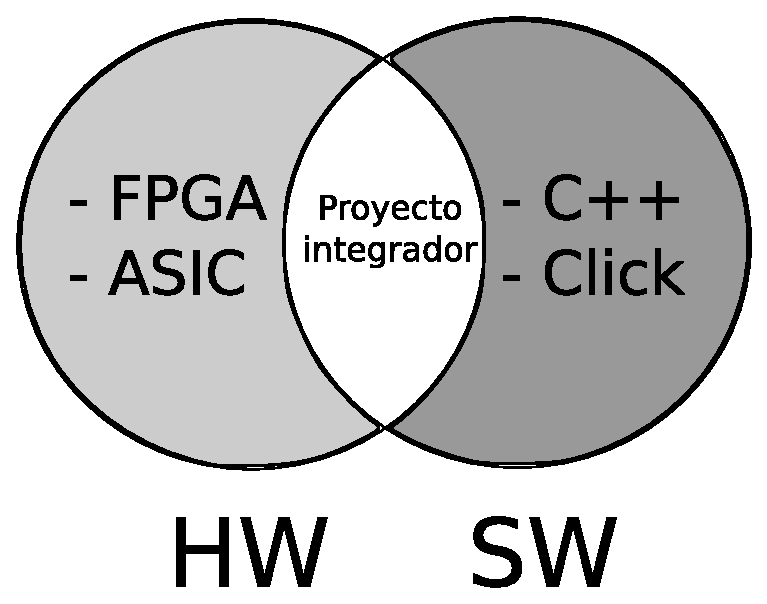
\includegraphics[width=0.6\textwidth]{2-sistema/graf/interseccion.eps}
  \caption{Arquitectura mixta}
  \label{fig:hwsw}
\end{figure}


\section{Solución propuesta}

Para el problema de clasificación planteado en el capítulo anterior se propone, de manera funcional, la siguiente solución: 

    \begin{enumerate}
  	\item Un flujo de paquetes llega a la interfaz de red del dispositivo y es necesario clasificarlo en distintos flujos para que sea redireccionado.
	\item Se almacenan los paquetes en un buffer según el orden de llegada.
	\item Se extrae el primer paquete y se toma la información que pertenece a la cabecera; La información completa del paquete queda en espera.
	\item Se envía la cabecera al microprocesador.
	\item El microprocesador aplica un algoritmo de clasificación a cierta información de la cabecera y reenvía los resultados al hardware. 
	\item Se envía el paquete a la interfaz de salida, anexándole a cada palabra un tag adjunto con el resultado de la clasificación.
    \end{enumerate}

\section{Esquema propuesto}
Para implementar la solución se propone el hardware descripto en el diagrama de la figura~\ref{fig:solucion}.
 \begin{figure}[h]
  \centering
	 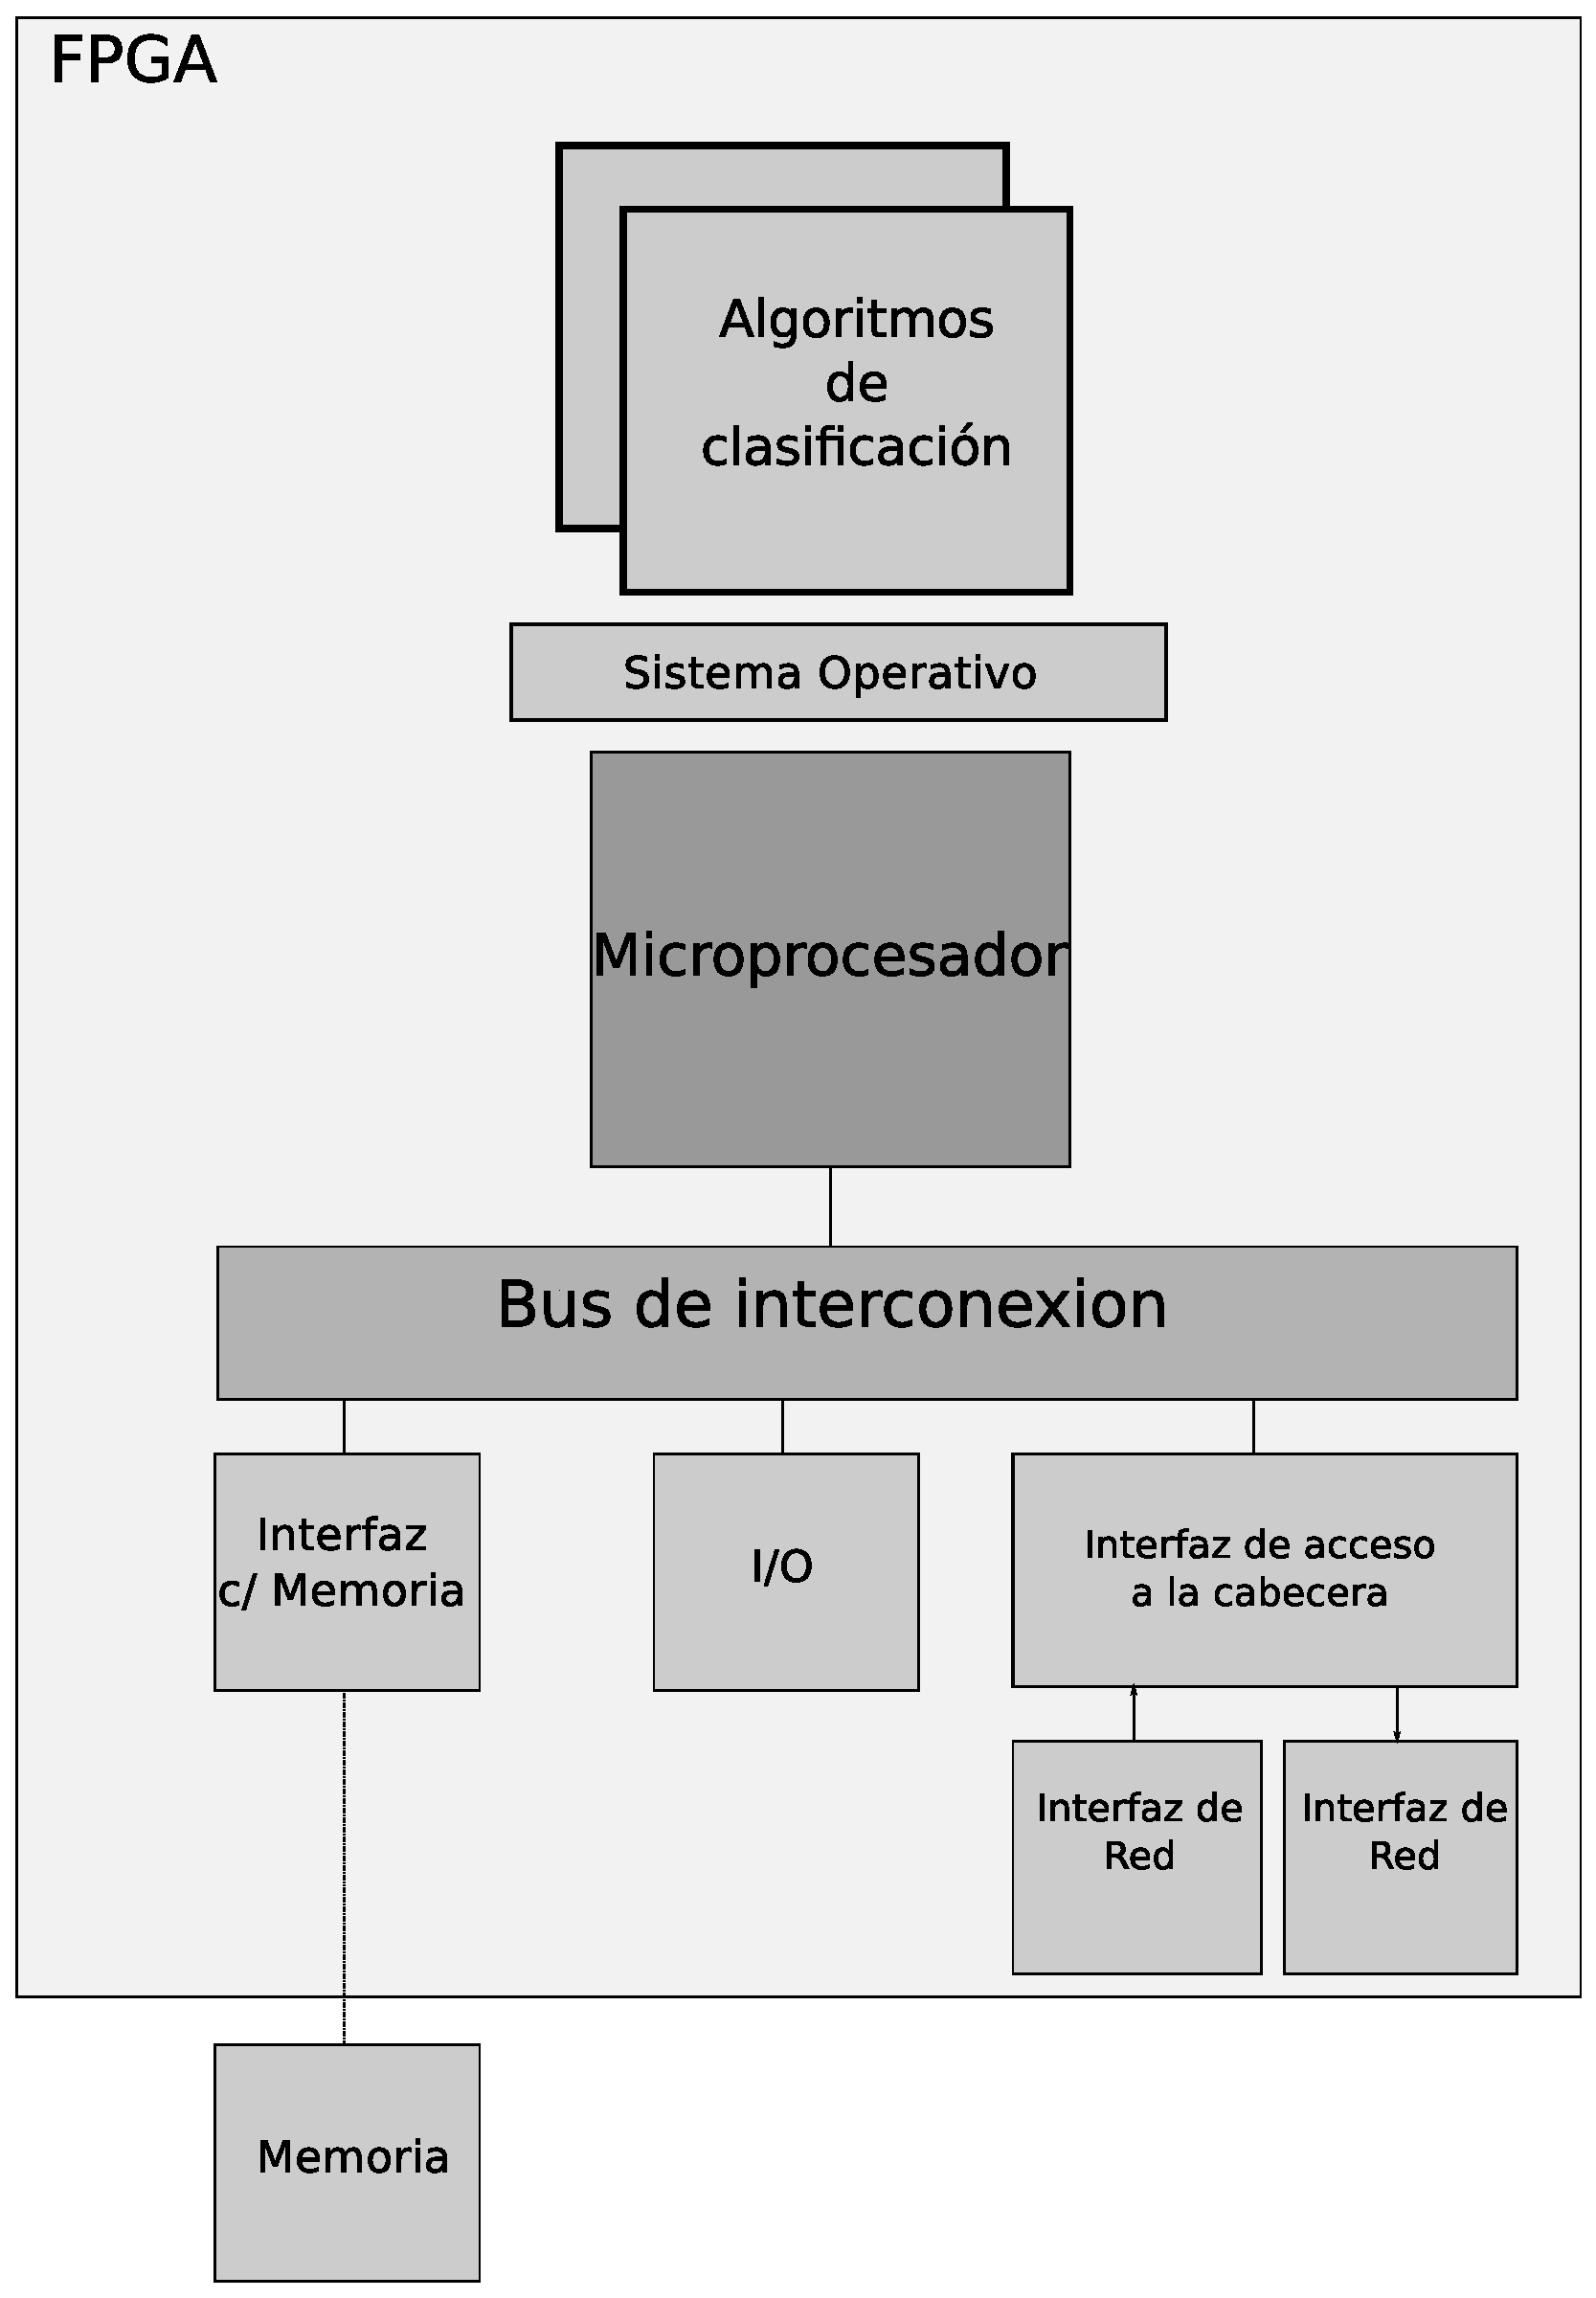
\includegraphics[width=0.6\textwidth]{2-sistema/graf/solucion.eps}
  \caption{Diagrama de la arquitectura propuesta}
  \label{fig:solucion}
\end{figure}

De los módulos mencionados, es necesario poner especial atención en el diseño de la interfaz de acceso a la cabecera.

\subsection{Interfaz de acceso a la cabecera}
Este módulo tiene como función acceder a los campos que conforman la cabecera IP en los paquetes entrantes. En este caso el hardware realiza esencialmente funciones de transferencia de paquetes. La información recolectada es enviada al microprocesador para que éste implemente el software de clasificación.

\newpage

 \begin{figure}[h]
  \centering
	 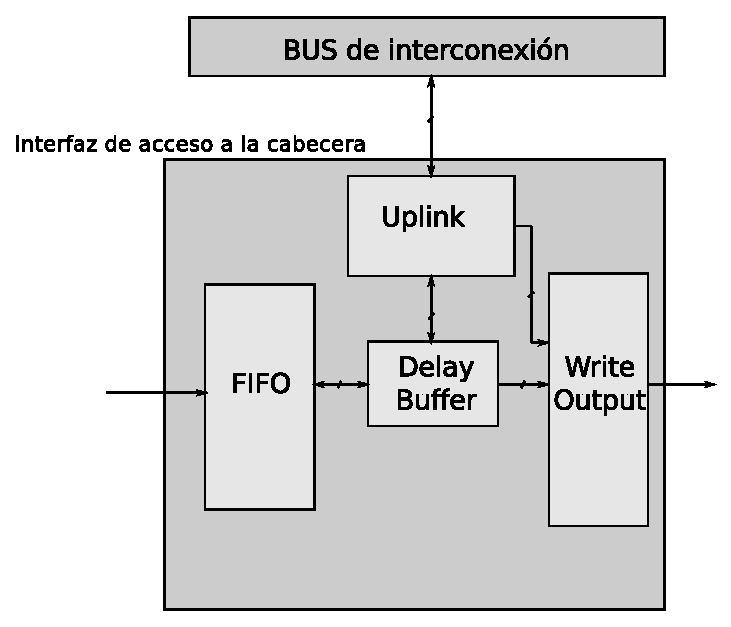
\includegraphics[width=0.6\textwidth]{2-sistema/graf/modulo.eps}
  \caption{Interfaz de acceso a la cabecera}
  \label{fig:inter}
\end{figure}



%\subsection{Descripción funcional}

A continuación se describe funcionalmente cada uno de los bloques que conforma la interfaz, ilustrada en la figura~\ref{fig:inter}
\subsubsection{Cola de espera FIFO\textit{(First in First out)}}
A la entrada del módulo se encuentra una FIFO que se encarga de almacenar y poner a disposición en orden de llegada los datos de entrada, que pueden venir de un generador o de otra etapa de procesamiento, como ser la que se lleva a cabo en una interfaz de red. Además, para poder manipular los paquetes, la FIFO debe almacenar toda la información de control disponible a su entrada.
Este módulo también debe permitir la parametrización en la mayor cantidad de sentidos posibles, especialmente se desea poder configurar la cantidad de palabras a almacenar, ya que la memoria dentro de un FPGA es un recurso crítico y se debe encontrar la mejor relación entre rendimiento y consumo de recursos.

\subsubsection{Delay Buffer}
Este componente será el encargado de ir tomando los datos desde la FIFO y de detectar el inicio y finalización de un paquete. Además deberá mantener almacenada la cabecera del paquete mientras el software toma una decisión. En este módulo es deseable configurar la cantidad de palabras que se considerarán parte de la cabecera y que serán enviadas al microprocesador.

\subsubsection{Uplink}
Este módulo es el encargado de gestionar las transacciones con el microprocesador. Para ello debe entender las señales que utiliza el bus y poder interrumpir al procesador para enviarle los datos cuando estos estén disponibles. Asimismo cuando el procesador responde con el resultado de la clasificación, Uplink lo almacena y lo envía al módulo Write Output para que éste escriba el resultado de la clasificación en la etiqueta anexa al paquete correspondiente.
Eventualmente se desarrollarán varias versiones de este módulo, que envíen toda la cabecera o una parte selectiva de ella buscando optimizar el rendimiento.

\subsubsection{Write Output}
Para finalizar este módulo toma la salida de Delay Buffer y escribe el resultado que le envía Uplink en la etiqueta que se encuentra anexa a cada una de las palabras del paquete.

\section{Algoritmos de Clasificación}

Los algoritmos de clasificación de paquetes que se implementaron fueron los siguientes:

\subsection{Búsqueda lineal}

El esquema más simple de lookup consiste en una tabla, donde cada entrada contiene un prefijo (expresado en notación máscara) mas un identificador de enlace de salida. Cuando llega un paquete se examina su dirección IP y se va comparando con cada uno de los prefijos almacenados. Para que exista correspondencia debe existir igualdad bit a bit entre el prefijo y la dirección IP. Si esto se cumple para varios prefijos, se opta por el más largo de ellos y el paquete se expide por el enlace asociado a dicho prefijo.
Para optimizar este esquema, los prefijos se almacenan en orden decreciente de longitud, como se muestra en la figura~\ref{fig:linear}, de manera que al encontrar una coincidencia no sea necesario seguir buscando en el resto de la tabla. 

\begin{figure}[h]
  \centering
	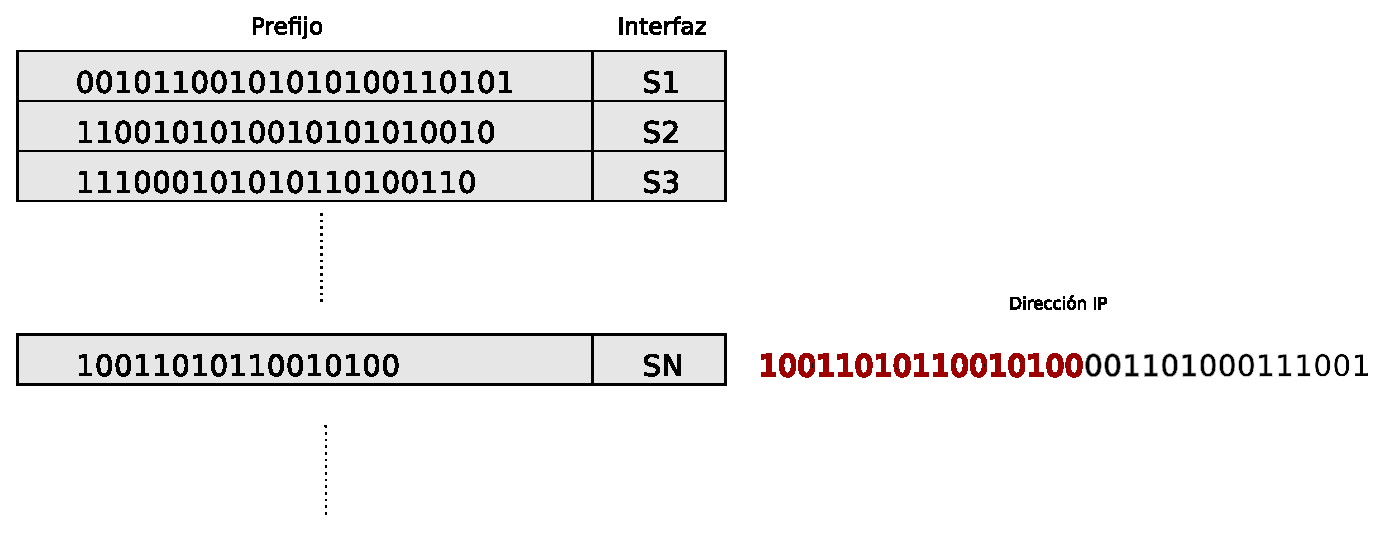
\includegraphics[width=0.80\textwidth]{2-sistema/graf/linear.eps}
  \caption{Búsqueda lineal}
  \label{fig:linear}
\end{figure}

\newpage
\subsection {Unibit tries}

Un Unibit trie es un árbol en el cual cada nodo contiene un \textit{puntero-cero }y un \textit{puntero-uno}. Partiendo del nodo raíz, todos los prefijos que comienzan con 0 son almacenados en el subárbol apuntado por el puntero-cero y aquellos que comienzan con 1 se almacenan en el subárbol apuntado por el puntero-uno. Cada subárbol es construido recursivamente de manera similar usando los bits restantes de cada uno de los prefijos.
Considerar la siguiente tabla de enrutamiento:
\begin{table}[h]
\begin{center}
	\begin{tabular}{|c|c|} \hline
		\textbf{Prefijo} & \textbf{Enlace de salida} \\ \hline
		101* & S1 \\
		111* & S2 \\
		11001* & S3 \\
		1* & S4 \\
		0* & S5 \\
		1000* & S6 \\
		100000* & S7 \\
		100* & S8 \\
		110* & S9 \\	\hline
	\end{tabular}
	\caption{Prefijos y enlaces de salida}
	\label{tab:prefgw}	
\end{center}
\end{table}



A la misma le corresponde la representación en Unibit trie de la figura~\ref{fig:trie}.
Sea una dirección de destino \textit{D}. Para efectuar la búsqueda del prefijo más largo, los bits de \textit{D} son usados para trazar un camino a lo largo del trie. Dicho camino comienza en el nodo raíz y continúa hasta encontrar un puntero vacío o un nodo vacío. Durante el recorrido a través del trie, el algoritmo mantiene un registro del último enlace encontrado en un nodo del camino recorrido (que es el mas largo hasta el momento). En el caso que la búsqueda terminara éste es el prefijo retornado.

\begin{figure}[h]
  \centering
	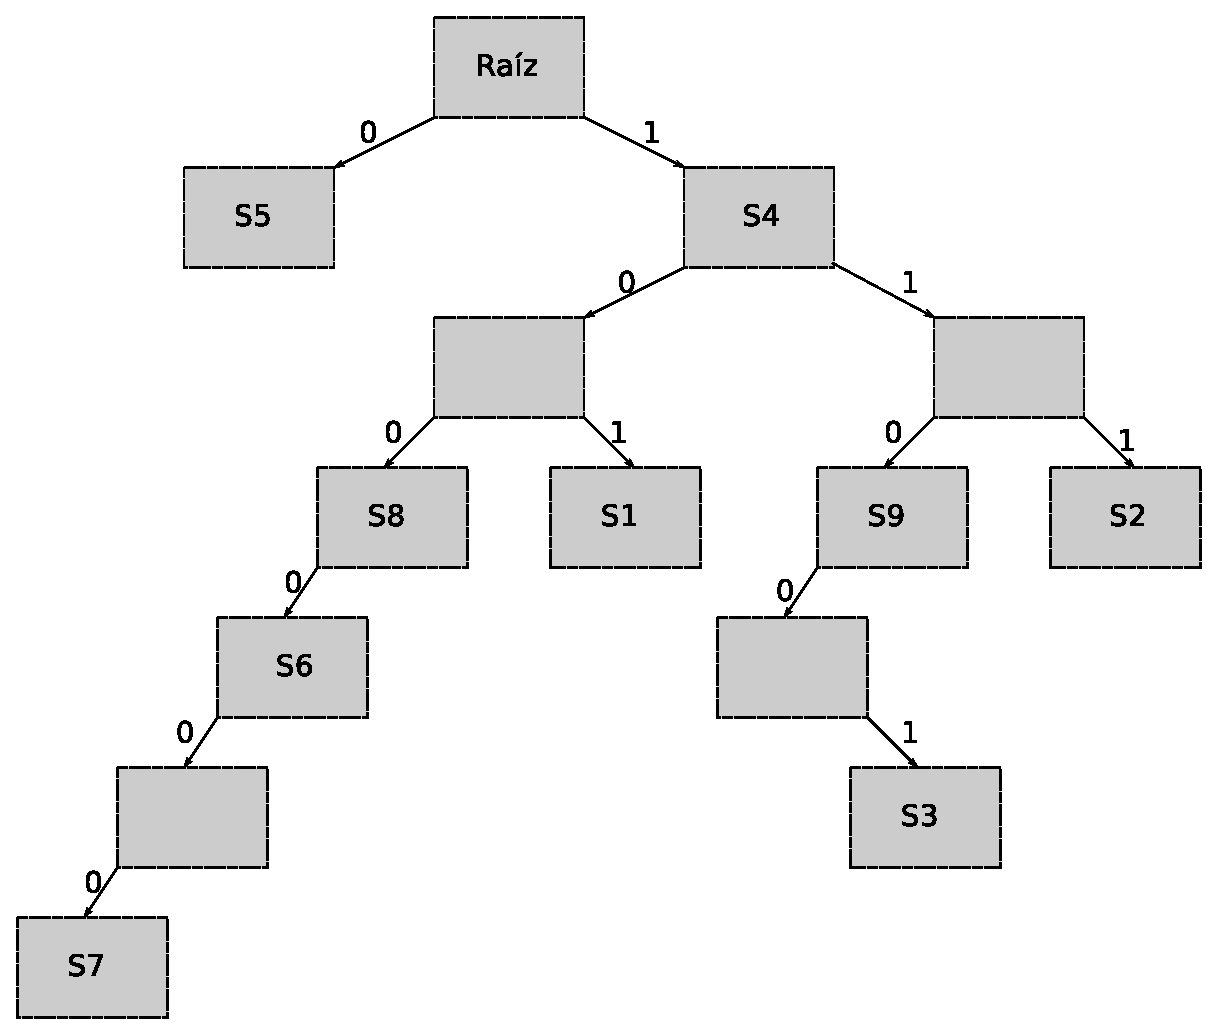
\includegraphics[width=0.80\textwidth]{2-sistema/graf/trie.eps}
  \caption{Unibit trie}
  \label{fig:trie}
\end{figure}


 
\chapter{Arquitectura}
En este capitulos se detallara la arquitectura del proyecto en general, poniendo foco en la seleccion adecuada de las tecnologias a utilizar y completando mas detalladamente el diseño obtenida en el capitulo anterior.

\section{Procesador Embebido}

Como se dijo en el capitulo 2, los microprocesadores embebidos en logica reprogramable se clasifican, basicamente, en dos tipos Hardcore y Softcore. Aunque los Hardcores ofrecen unas mejores prestaciones existen muy pocos dispositivos en el mercado que ofrecen este tipo de modulos y, en general, el costo de este tipo de dispositivos es mayor que el de uno que no cuenta con un hardcore. Por esta razones de ahora en adelante se limitara el estudio a softcores, siempre buscando que lo implementado siga los principios del diseño modular a los fines de facilitar la portabilidad.
\subsection{Estudio de los softcores disponibles}
Los SoftCores pueden ser clasificados en tres tipos segun su origen

\begin{itemize}
	\item Provistos por los fabricantes de las FPGA
	\item Provistos por empresas distribuidoras de bloques IP(Intelectual Property)
	\item Provistos por la comunidad Open Source
\end{itemize}

\subsubsection{Provistos por los fabricantes de las FPGA}
Xilinx y Altera, los dos mayores fabricantes de FPGA, proveen un Softcore para integrar en sus dispositivos. La ventaja natural de este tipo de core es que se encuentran altamente integrados en las herramientas de desarrollo de dichos fabricantes, permitiendo montar un sistema embebido en minutos de manera grafica e intuitiva. Ademas estan a disposición del usuario una buena cantidad de  modulos IP para anexar al procesador y aumentar asi sus funcionalidades. 

Dentro de las desventajas esta el hecho de que son dependientes de la plataforma y no es posible implementar el core propietario de Altera en un dispositivo Xilinx, y viseversa. Ademas se debe pagar una licencia por el uso de estos cores y no se cuenta con la posibilidad de observar o modificar el codigo de los mismos. 

Xilinx ofrece a los usuarios de sus dispositivos el MicroBlaze, un procesador RISC de 32 bits con una arquitectura muy similar al MIPS DLX. A nivel herramientas de desarrollo la empresa provee el "Xilinx's EDK(Embedded Development Kit)" que permite generar un sistema embebido completo con las interconexiones necesarias. Es posible correr el sistema operativo GNU/Linux en este tipo de procesador.

Altera por su parte ofrece la linea de Cores NIOS II, tambien RISC de 32 bits, que cuenta en tres variantes principales Nios II Fast, Economy y Standard y dos variantes especializadas Nios II SC core, para aplicaciones militares y aeroespaciales, y DesignWare IP, para implementar en ASIC. Altera provee ademas una interfaz de usuario para la construccion del sistema embebido llamado SOPC que se encuentra integrado a Quartus y ademas el Nios II Embedded Design Suite (EDS) que permite diseñar el software requerido para cada aplicacio. Permite la implementacion del sistema operativo GNU/Linux.

\subsubsection{Provistos por empresas distribuidoras de bloques IP}
Existe una buena cantidad de empresas que se dedican a generar y comercializar bloques de propiedad intelectual (IP Cores o IP Blocks), unidades logicas reusables que son propiedad intelectual de un individuo o empresa.
Varias de estas empresas cuentan con Softcores con distintas capacidades y tecnologias. La ventaja principal esla portabilidad de estos cores entre FPGA de distintos fabricantes. Entre las desventajas podemos nombrar la calidad de la documentacion y la complejidad intrinseca que implica comprender y utilizar una herramienta de desarrollo de un tercero. 

Dentro de los mas conocidos se puede nombrar a la linea Leon de la empresa Aeroflex, LatticeMico32 de Lattice semiconductor o ARM cortex de Freescale. Los IP core pueden estar licenciados de diferentes formas incluidas entre ellas GPL.
 
\subsubsection{Provistos por la comunidad Open Source}
La comunidad open source se ha encargado de producir una buena cantidad de softcores, las capacidades y perfomance de los mismos cubre casi todos los rangos. En la pagina web que lleva una lista de este tipo de proyectos, opencores, se pueden encontrar alrededor de 130 cores. El problema con este tipo de core esta en la poco uniforme calidad de la documentacion y en la calidad dudosa de varios de los cores. Sin embargo la flexibilidad para poder modificar la arquitectura a gusto y el costo cero de implementacion son ventajas nada despreciables de estos productos. 

Se destaca el proyecto Openrisc 1200, que tiene una gran comunidad que lo soporta y algun prestigio ganado en este terreno.


\subsubsection{Tabla comparativa}
																																						 \newpage																												
\begin{table}
	\center
	\begin{tabular}{|p{1.65cm}|p{1.98cm}|p{1.9cm}|p{2.2cm}|p{1.5cm}|c|c|p{1.5cm}|} \hline
		Core & Arquitectura & Licencia & Profundidad del Pipeline & Ciclos por Instruccion & MMU & FPU & FPGA \\ \hline
		MicroBlaze & MicroBlaze & Propietaria & 3,5 & 1 & Opt & Opt & Xilinx\\ \hline
		Nios II/fast & Nios II & Propietaria & 6 & 1 & si & opt & Altera \\ \hline
		Nios II/std & Nios II & Propietaria & 5 & 1 & no & Opt & Altera \\ \hline
		Nios II/econ & Nios II & Propietaria & no & 6 & no & Opt & Altera \\ \hline
		LEON3 & SPARC-v8 & Open Source(GPL) & 7 & 1 & si & si & Xilinx, Altera, Lattice \\ \hline
		OpenRISC 1200 & OpenRISC 1000 & Open Source(LGPL) & 5 & 1 & si & no & Xilinx, Altera, Lattice \\ \hline
		Lattice Mico32 & Lattice Mico32 & Open Source & 6 & 1 & no & no & Indep. \\ \hline
		Cortex-M1 & ARMv6 & Propietaria & 3 & 1 & no & no & Xilinx, Altera \\ \hline
	\end{tabular}
	\caption{Comparativa softcores}
	\label{tab:comp}
\end{table}

\subsection{Criterios de Seleccion}

Los criterios mas importantes a la hora de seleccionar el Softcore que va a ser utilizado en este proyecto son:
\begin{itemize}
	\item Hardware: se debe contar con el dispositivo necesario para la implementacion de estos dispositivos.
	\item Herramientas de Diseño: la cadena de herramientas necesarias para diseñar el sistema y el software debe ser simple y funcional, para evitar que comprender las herramientas lleve mas tiempo que realizar el proyecto en si mismo.
	\item Rendimiento: se desea que el rendimiento sea aceptable y que sea posible optimizarlo a medida de que el proyecto avanza.
\end{itemize}

Bajo estos criterios y teniendo en cuenta que en el laboratorio en que se realiza el presente proyecto integrador es posible acceder a una amplia variedad de kits de desarrollo equipados con FPGAs de Altera, todas las licencias de software y varios proyectos con antencedentes de haber puesto en funcionamiento un Nios II es este el Core seleccionado para el sistema embebido a implementar.

\subsection{Nios II}
El Nios II es un procesador RISC de 32 bits de proposito general que cuenta con las siguientes especificaciones:
\begin{itemize}
	\item Set de instrucciones, bus de datos y espacio de direcciones de 32 bits.
	\item 32 registros de proposito general.
	\item Soporte para hasta 32 interrupciones.
	\item Controlador de interrupciones externas para soportar una mayor cantidad de interrupciones.
	\item Multiplicacion y division en una sola instruccion de 32 x 32 produciendo un resultado de 32-bits.
	\item Instrucciones dedicadas para multiplicaciones con resultados de 64 y 128 bits.
	\item Acceso a una variedad de perifericos e interfases a memorias  y perifericos fuera del chip.
	\item Modulo de depurado asistido por hardware.
	\item Unidad de manejo de memoria (MMU) opcional para soportar sistemas operativos mas complejos.
	\item Unidad de proteccion de memoria (MPU) opcional.
	\item Entorno de desarrollo de software basado en GNU C/C++ integrado a Eclipse.
	\item Integracion con SignalTap® II, el analizador de logica embebida de altera permitiendo el analisis de tiempo real de todas las señales presentes en la FPGA.
	\item Set de instrucciones compatible entre todos las versiones del procesador Nios II.
\end{itemize}


\subsection{SOPC}
\section{Modulo Gestor de Datos}
\section{Software}

\subsection{NIOS II SBT}

El NIOS II Software Building Tools (o SBT) es un conjunto de utilidades y scripts que sirve para crear y construir aplicaciones embebidas basadas en C/C++, librerías de usuario y paquetes de soporte de placa (board support packages o BSP). 

Puede invocarse desde la IDE Eclipse o desde el intérprete de comandos del NIOS II.

El NIOS II SBT puede crear los siguientes tipos de proyecto:
\begin{itemize}
	\item Aplicación NIOS II: un programa que implementa alguna funcion deseada.
	\item NIOS II BSP: una librería que provee acceso al hardware en el sistema. Brinda un entorno de rutinas a medida para un procesador y, eventualmente, un sistema operativo. 
	\item Librería de usuario: un conjunto de funciones reutilizables. 
\end{itemize}

\subsubsection{Aplicaciones y librerías de usuario}

Para el caso de aplicaciones y librerías de usuario, el SBT genera un makefile privado (denominado \textbf{Makefile}) el cual es usado para construir el proyecto. Al hacer esto se genera un archivo .elf para una aplicación, o .a para una librería. En este último caso, también se produce un makefile público (denominado \textbf{public.mk}), que se incluye en el privado para cualquier aplicación que use la librería de usuario.

Cuando se crea un makefile se provee al SBT con una lista de archivos de código fuente y una referencia al directorio donde se almacena el BSP. Luego, la herramienta examina la extensión de cada archivo fuente para determinar el lenguaje de programación. 

Actualmente, los soportados son:

\begin{itemize}
	\item C (extensión .c).
	\item C++ (extensiones .cpp, .cxx, .cc).
	\item NIOS II Assembler (extensiones .s, .S).
\end{itemize}


\subsubsection{Board Support Packages}

Un BSP es una librería especializada que contiene código de soporte específico del sistema. Aisla la aplicación de los detalles del sistema, tales como mapeo de memoria, dispositivos disponibles y configuración del procesador.

Se compone de:

\begin{itemize}
	\item Capa de abstracción de Hardware (Hardware Abstraction Layer o HAL): Permite al software interactuar con el hardware del sistema. Se describirá en detalle más adelante en este capítulo.
	\item Librería C estándar newlib: ANSI C estándar diseñada para sistemas embebidos.
	\item Drivers de dispositivos: para manejar cada uno de los componentes del sistema.
	\item Paquetes de software opcionales: permiten proveer funcionalidad adicional.
	\item Sistema operativo de tiempo real opcional: implementación de MicroC/OS-II RTOS.
\end{itemize}

\subsubsection{Proceso de construcción del software}

Para crear un proyecto de software se llevan a cabo una serie de pasos:

\begin{enumerate}
	\item Se obtiene el diseño de hardware sobre el cual va a correr el software. Dicha información está almacenada en un archivo de extensión \textbf{.sopcinfo}, el cual es generado por la herramienta SOPC builder.
	\item Se genera el BSP con las características necesarias según las funcionalidades requeridas. También se genera un makefile para dicho paquete.
	\item Opcionalmente, se crea una librería de usuario (junto a su correspondiente makefile).
	\item Se escribe el software de aplicación. Se colecta todo el código fuente, y luego se genera el makefile correspondiente.
	\item Se construye el proyecto.
\end{enumerate}


\subsection {HAL}

La Capa de Abstracción de Hardware \textit{(Hardware Abstraction Layer o HAL)} provee una interfaz simple de drivers de dispositivos para conectar los programas con el hardware subyacente. La API está integrada con la librería estándar ANSI C, lo cual permite al software acceder a los dispositivos mediante el uso de funciones C ampliamente conocidas, tal como printf(), fopen(), fwrite(), etc.

\subsubsection{Servicios}

La HAL provee los siguientes servicios:

\begin{itemize}
	\item Integración con la librería estándar newlib: provee funciones estándar ANSI C de amplio uso.
	\item Drivers de dispositivo: brinda acceso a cada dispositivo en el sistema.
	\item API: proporciona una interfaz estándar consistente a los servicios de la HAL, tales como acceso a dispositivos y manejo de interrupciones.
	\item Inicialización de sistema: Lleva a cabo la inicialización para el procesador y las rutinas antes de ejecutar la función principal (main).
	\item Inicialización de dispositivos: Instancia e inicializa cada uno de los dispositivos del sistema antes de que se ejecute la función main.
\end{itemize}

La figura ~\ref{fig:hal} muestra las capas de un sistema basado en la HAL, desde el nivel de hardware hasta el programa de usuario.

\begin{figure}[H]
  \centering
	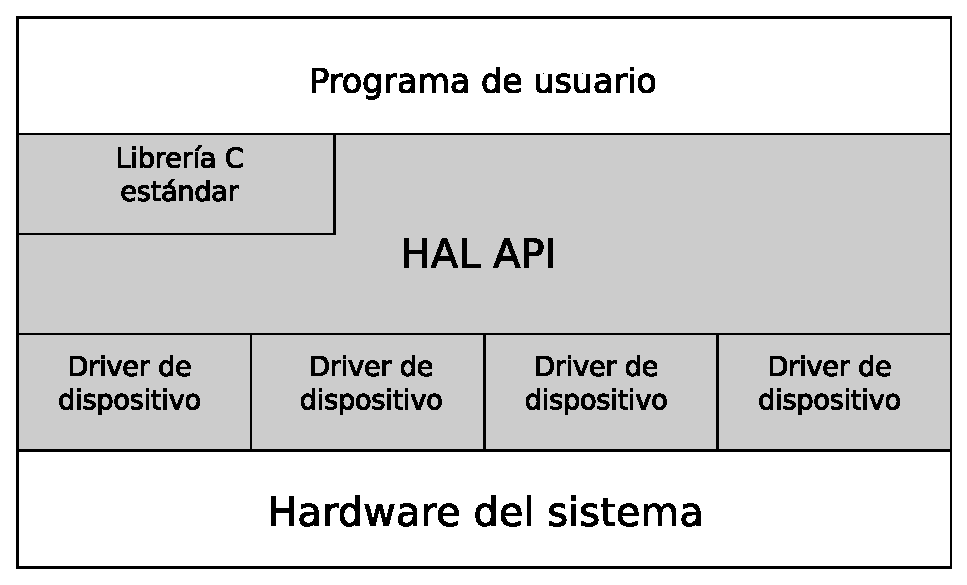
\includegraphics[width=0.80\textwidth]{3-arquitectura/graf/hal.eps}
  \caption{Capas de un sistema basado en la HAL.}
  \label{fig:hal}
\end{figure}

\subsubsection{Modelos de dispositivos genéricos}

La HAL provee modelos de dispositivos genéricos para diversos tipos de periféricos que se encuentran en sistemas embebidos, tales como timers, interfaces Ethernet y dispositivos de I/O que transmiten datos de caracter. Estos modelos permiten escribir programas usando una API consistente sin preocuparse por el hardware subyacente.

Los tipos de periféricos cubiertos son:

\begin{itemize}
	\item Dispositivos de caracter: envían y/o reciben caracteres en forma serial, como ser una UART.
	\item Timers: dispositivos que llevan la cuenta de los tics de un clock y pueden generar interrupciones periódicas.
	\item Subsistemas de archivos: un mecanismo para acceder a archivos almacenados en dispositivos físicos. Dependiendo de la implementación interna, el driver del subsistema de archivos podría acceder a los dispositivos subyacentes en forma directa o usar un driver aparte.
	\item Dispositivos Ethernet: proveen acceso a una conexión Ethernet para una pila de red, tal como la NicheStack® TCP/IP Stack, provista por Altera.
	\item Dispositivos DMA: periféricos que llevan a cabo una gran cantidad de transacciones de datos. El origen y destino pueden ser la propia memoria o algún otro dispositivo.
	\item Dispositivos con memoria flash: periféricos con memoria no volátil que utilizan un protocolo especial de programación para almacenar datos.
\end{itemize}

Todos los periféricos, ya sean de Altera o de terceros, deben proveer un archivo de cabecera que defina la interfaz de bajo nivel del dispositivo con el hardware. 

Ciertos dispositivos tienen características específicas de hardware con requierimientos de uso que no se adaptan bien a una API de propósito general. La HAL maneja dichos requerimientos mediante la función ioctl(), cuyas opciones dependerán del periférico en cuestión.

Algunos periféricos proveen funciones de acceso dedicadas que no están basadas en el modelo genérico de la HAL. En ese caso, se debe proveer un archivo de cabecera con dichas funciones.


\subsubsection{Librería C estándar : newlib}
La HAL integra su entorno de rutinas con una implementación open-source de la librería C estándar:\textbf{ newlib}. La misma está hecha para ser utilizada en sistemas embebidos. 

\subsubsection{La HAL dentro de un proyecto de software}
La creación y administración de proyectos basados en la HAL están altamente ligadas al NIOS II SBT

\begin{figure}[h]
  \centering
	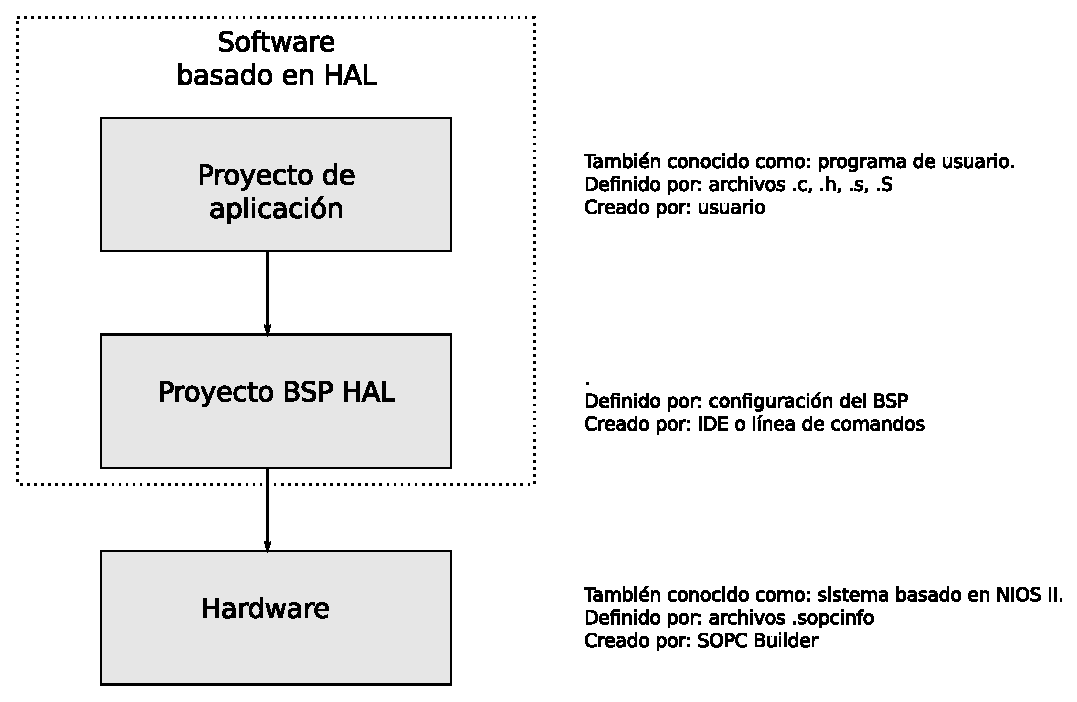
\includegraphics[width=0.90\textwidth]{3-arquitectura/graf/halsof.eps}
  \caption{Capas de un programa basado en HAL}
  \label{fig:halsof}
\end{figure}

La figura ~\ref{fig:halsof} muestra el diagrama en bloques de un software basado en la HAL. Todo programa de este tipo consta de dos proyectos. El ćodigo de aplicación específico se encuentra en uno de ellos, el cual depende a su vez de otro proyecto BSP separado.

EL primero contiene todo el código que el programador desarrolla. El segundo, toda la información necesaria para la interacción hardware-software. Este último a su vez depende del hardware del sistema, cuya información se encuentra en un archivo generado por la herramienta SOPC Builder.

\subsubsection{El archivo de descripción del sistema (system.h)}
El archivo system.h provee una descripción completa del software del sistema basado en NIOS II. Describe cada periférico e incluye:

\begin{itemize}
	\item La configuración de hardware del periférico.
	\item La dirección base.
	\item Información IRQ (si es necesario).
	\item Un nombre simbólico para el periférico.
\end{itemize}

El SBT genera un archivo \textbf{system.h} para cada proyecto BSP, cuyo contenido dependerá del archivo .sopcinfo mencionado anteriormente en este capítulo.



La razón de utilizar la HAL en vez de un sistema operativo, yace principalmente en la mayor simplicidad de uso que ésta presenta. En el caso de haber optado por el segundo enfoque hubiese sido necesario el desarrollo de drivers para el manejo de los dispositivos, con la complejidad que ello implica. La HAL, por otra parte, ofrece un conjunto de funciones de la librería estándar ANSI C para la interacción con el hardware del diseño, lo cual hace que dicha tarea sea significativamente más simple.



\subsection {Algoritmos de clasificación}

Se implementaron 2 algoritmos de clasificacion: Busqueda lineal y Busqueda en árbol unibit.

El software utilizado para realizar las pruebas consistió en 2 proyectos por separado. Uno para cada tipo de búsqueda en la tabla.

El mismo fue desarrollado en lenguaje c++, por presentar éste ciertas facilidades para las implementaciones llevadas a cabo. Puntualmente se sacó ventaja de un STL container (list) para implementar la búsqueda lineal. La característica utilizada en este caso fue el ordenamiento de la lista con sólo una llamada a función.

Para efectuar el intercambio de datos con el hardware se hizo uso de las macros IOWR e IORD, las cuales escriben y leen respectivamente los datos hacia/desde un componente conectado al bus Avalon MM. La razón de haber usado dichas macros yace en el hecho de que las mismas no son puestas en caché. Esta característica se torna indispensable en este diseño, ya que en el mismo no se puede leer un dato sin saber si está verdaderamente disponible en el bus.


\subsubsection {Búsqueda lineal}

Se implementó en una lista enlazada, creada a partir del template list de c++. Los nodos de la lista contienen 3 campos:

\begin{itemize}
	\item Dirección de red (entero de 32 bit sin signo)
	\item Máscara de red (entero de 32 bit sin signo)
	\item Identificador de decisión (entero de 32 bit con signo)
\end{itemize}

Como se le dió prioridad a los prefijos de red más largos, se debió sobrecargar el operador de comparación ( > ) para que la función sort pudiese ordenar en base a la longitud de máscara. De esa manera, los nodos que contenían valores de máscara más grandes quedaban en las primeras posiciones de la lista.

Cuando la función encargada del lookup recibe una dirección IP de destino, realiza los siguientes pasos:

\begin{itemize}
	\item Coloca un iterador al comienzo de la lista.
	\item Realiza un AND con el valor de máscara del nodo que está siendo apuntado. Si el resultado de la operación es igual al valor de dirección de red de dicho nodo, entonces se retorna con el valor identificador de decisión. En otro caso, continúa la busqueda en el siguiente nodo.
\end{itemize}

\subsubsection {Busqueda en Arbol unibit}

Se implementó una clase en la cual se definieron las características de los nodos del arbol, como así tambien las operaciones de inserción y búsqueda.

En este contexto, pueden existir 2 tipos de nodo:

\begin{itemize}
	\item Común: no está asociado a una decisión.
	\item Decisión: contiene un valor que identifica a la decisión a tomar. 
\end{itemize}

Cada nodo cuenta con los siguientes campos:
\begin{itemize}
	\item gw: es un identificador de la decisión a tomar. En los nodos no asociados a una decision, tiene el valor estipulado en la macro NONE.
    \item zero / one: Son punteros a nodo, asociados a los bits 0/1 del prefijo que se esté leyendo.

\end{itemize}




El algoritmo de búsqueda toma como entrada la dirección IP de destino del paquete a clasificar. Luego de ello, va haciendo un testeo bit a bit de la misma, partiendo con un puntero de recorrido desde el nodo raíz. Si el bit de la dirección es 0 y el puntero zero está apuntando hacia algun nodo, el puntero de recorrido se mueve al nodo apuntado por el puntero zero. En caso contrario, se mueve al nodo apuntado por el puntero one (En caso de que exista alguno). Esto se repite nodo a nodo, hasta que ocurre alguna de las siguientes situaciones:

\begin{itemize}
    	\item     El puntero de recorrido queda varado en un nodo decision, con lo cual se retorna el valor de gw.
    	\item El puntero de recorrido queda varado en un nodo común. 
\end{itemize}



Contemplando esta última posibilidad, el algoritmo hace que en cada nodo se chequee si se trata de un nodo decisión. En dicho caso, se almacena el campo gw en una variable y se continua el recorrido. Si se da un caso en el cual el nodo de recorrido queda apuntando a un nodo comun y luego de testear un bit se determina que el mismo no tiene un nodo asociado (es decir, que alguno de los punteros zero / one esté en NULL) la funcion retorna la variable anteriormente mencionada. 

\subsection {Cache}

Se implementó una cache directa. La misma consta de una tabla hash de 16 entradas. Las colisiones se resuelven por reemplazo directo. La misma fue testeada con ambos algoritmos mencionados anteriormente. Para ello, se agregó una lógica adicional que consistió en:

\begin{itemize}
	\item Al tomar una direccion IP, chequear primero si el valor de decisión se encuentra en caché.
	\item Si está, retornar dicho valor.
	\item En otro caso, efectuar el lookup y almacenar el valor de decisión en caché.
\end{itemize}

Para evitar el overhead introducido por el uso de clases, se optó por el uso de estructuras para la implementación de este último enfoque.

\begin{comment}
\section{Parte HW}

\subsection{Componentes del sistema}

\subsubsection*{NIOS II}

Es un microprocesador softcore. Esto significa que el mismo es instanciado usando la lógica propia de la FPGA. En este diseño, ejecuta un software de clasificación de paquetes que se almacena en una memoria SDRAM en la placa de desarrollo.

\subsubsection*{PLL}

Este módulo toma como entrada una señal de clocl de 50 MHZ de frecuencia y la bifurca en 2: Una de ellas alimentará al módulo que oficia de interfaz con la memoria SDRAM y la otra hará lo propio con el resto de los componentes del sistema. Estas señales están defasadas entre sí 60º con el fin de evitar el skew producido por la diferencia entre la llegada del clock a la memoria y al resto del sistema.

\subsubsection*{Timer}

Módulo utilizado para llevar estadísticas de retardo dentro del software.

\subsubsection*{JTAG UART}

Este módulo permite interactuar con el sistema vía USB. Esto implica tanto la configuracion de la FPGA, como también la posibilidad de ver la ejecución del software en una consola.

\subsubsection*{Interfaz con SDRAM}

Tiene la función de interconectar al sistema con la memoria SDRAM de la placa de desarrollo.

\subsubsection*{Extractor de cabeceras}

Este módulo extrae cabeceras de paquetes Ethernet y las envía al software, donde son procesadas y devueltas. Su funcionamiento se detallará a continuación.

\subsection{Módulo extractor de cabeceras}


(..esta parte completala vos...)

\section{Parte SW}

\section{Parte SW}

Se implementaron 2 algoritmos de clasificacion: Busqueda lineal y Busqueda en árbol unibit.

El software utilizado para realizar las pruebas consistió en 2 proyectos por separado. Uno para cada tipo de búsqueda en la tabla.

El mismo fue desarrollado en lenguaje c++, por presentar éste ciertas facilidades para las implementaciones llevadas a cabo. Puntualmente se sacó ventaja de un STL container (list) para implementar la búsqueda lineal. Esta plantilla cuenta con, entre otras cosas, la posibilidad de ordenar la lista con sólo una llamada a función.

Para efectuar el intercambio de datos con el hardware se hizo uso de las macros IOWR e IORD, las cuales escriben y leen respectivamente los datos hacia/desde un componente conectado al bus Avalon MM. La razón de haber usado dichas macros yace en el hecho de que las mismas no son "cacheadas". Esta característica se torna indispensable en este diseño, ya que en el mismo no se puede leer un dato sin saber si está verdaderamente disponible en el bus.


\subsection {Búsqueda lineal}

Se implementó en una lista enlazada, creada a partir del template list de c++. Los nodos de la lista contienen 3 campos:

\begin{itemize}
	\item Dirección de red (entero de 32 bit sin signo)

	\item Máscara de red (entero de 32 bit sin signo)

	\item Identificador de decisión (entero de 32 bit con signo)
\end{itemize}

Como se le dió prioridad a los prefijos de red más largos, se debió sobrecargar el operador de comparación ( > ) para que la función sort pudiese ordenar en base a la longitud de máscara. De esa manera, los nodos que contenían valores de máscara más grandes quedaban en las primeras posiciones de la lista.

Cuando la función encargada del lookup recibe una dirección IP de destino, realiza los siguientes pasos:

\begin{itemize}
	\item Coloca un iterador al comienzo de la lista.
	\item Realiza un AND con el valor de máscara del nodo que está siendo apuntado. Si el resultado de la operación es igual al valor de dirección de red de dicho nodo, entonces se retorna con el valor identificador de decisión. En otro caso, continúa la busqueda en el siguiente nodo.
\end{itemize}

\subsection {Busqueda en Arbol unibit}

Se implementó una clase en la cual se definieron las características de los nodos del arbol, como así tambien las operaciones de inserción y búsqueda.
Cada nodo cuenta con los siguientes campos:
\begin{itemize}
	\item gw: es un identificador de la decisión a tomar. En los nodos no asociados a una decision, tiene el valor estipulado en la macro NONE.
    \item zero / one: Son punteros a nodo, asociados a los bits 0/1 del prefijo que se esté leyendo.

\end{itemize}

En este contexto, pueden existir 2 tipos de nodo:

\begin{itemize}
	\item Común: Está asociado a la macro NONE. La misma lo diferencia del nodo decisión.
	\item Decisión: Contiene en el campo gw un valor que identifica a la decisión a tomar. 
\end{itemize}



El algoritmo de búsqueda toma como entrada la dirección IP de destino del paquete a clasificar. Luego de ello, va haciendo un testeo bit a bit de la misma, partiendo con un puntero de recorrido desde el nodo raíz. Si el bit de la dirección es 0 y el puntero zero está apuntando hacia algun nodo, el puntero de recorrido se mueve al nodo apuntado por el puntero zero. En caso contrario, se mueve al nodo apuntado por one (En caso de que exista). Esto se repite nodo a nodo, hasta que:

\begin{itemize}
    	\item     El puntero de recorrido queda varado en un nodo decision, con lo cual se retorna el valor de gw. Ó
    	\item El puntero de recorrido queda varado en un nodo común. 
\end{itemize}



Contemplando esta última posibilidad, el algoritmo hace que en cada nodo se chequee si se trata de un nodo decisión. En dicho caso, se almacena el campo gw en una variable y se continua el recorrido. Si se da un caso en el cual el nodo de recorrido queda apuntando a un nodo comun y luego de testear un bit se determina que el mismo no tiene un nodo asociado (es decir, que alguno de los punteros zero / one esté en NULL) la funcion retorna la variable anteriormente mencionada. 

\subsection {Cache}

Se implementó una cache directa. La misma consta de una tabla hash de 16 entradas. Las colisiones se resuelven por reemplazo directo. La misma fue testeada con ambos algoritmos mencionados anteriormente. Para ello, se agregó una lógica adicional que consistió en:

\begin{itemize}
	\item Al tomar una direccion IP, chequear primero si el valor de decisión se encuentra en caché.
	\item Si está, retornar dicho valor.
	\item En otro caso, efectuar el lookup y almacenar el valor de decisión en caché.
\end{itemize}
\end{comment}

%\section{Distribucion Lineal}

\chapter{Implementación}

\section{Algoritmos de clasificación}

Se implementaron 2 algoritmos de clasificación: Búsqueda lineal y Búsqueda en árbol unibit.

El software utilizado para realizar las pruebas consistió en 2 proyectos por separado. Uno para cada tipo de búsqueda en la tabla.

El mismo fue desarrollado en lenguaje c++, por presentar éste ciertas facilidades para las implementaciones llevadas a cabo. Puntualmente se sacó ventaja de un STL container (list) para implementar la búsqueda lineal. La característica utilizada en este caso fue el ordenamiento de la lista con sólo una llamada a función.

Para efectuar el intercambio de datos con el hardware se hizo uso de las macros IOWR e IORD, las cuales escriben y leen respectivamente los datos hacia/desde un componente conectado al bus Avalon MM. La razón de haber usado dichas macros yace en el hecho de que las mismas no son puestas en caché. Esta característica se torna indispensable en este diseño, ya que en el mismo no se puede leer un dato sin saber si está verdaderamente disponible en el bus.


\subsection {Búsqueda lineal}

Se implementaron 2 clases. 

\begin{itemize}
	\item \textit{iproute.h}: define el contenido de cada nodo de la lista (entrada en la tabla de ruteo).
	\item \textit{iplookup.h} -  contiene la lista que constituye la tabla de ruteo en sí, así como también las funciones de inserción y búsqueda. También contiene la función que crea una tabla de ruteo de 100 entradas.
\end{itemize}

Los nodos de la lista contienen 3 campos:

\begin{itemize}
	\item Dirección de red (entero de 32 bit sin signo)
	\item Máscara de red (entero de 32 bit sin signo)
	\item Identificador de decisión (entero de 32 bit con signo)
\end{itemize}

Como se le dio prioridad a los prefijos de red más largos, se debió sobrecargar el operador de comparación ( > ) para que la función sort pudiese ordenar en base a la longitud de máscara. De esa manera, los nodos que contenían valores de máscara más grandes quedaban en las primeras posiciones de la lista.

La función de inserción toma como entrada una dirección, una máscara y un identificador de decisión. Luego instancia una entrada con dichos elementos y la inserta en la lista.

Cuando la función encargada del lookup recibe una dirección IP de destino, realiza los siguientes pasos:

\begin{itemize}
	\item Coloca un iterador al comienzo de la lista.
	\item Realiza un AND con el valor de máscara del nodo que está siendo apuntado. Si el resultado de la operación es igual al valor de dirección de red de dicho nodo, entonces se retorna con el valor identificador de decisión. En otro caso, continúa la búsqueda en el siguiente nodo.
\end{itemize}

\subsection {Búsqueda en Árbol unibit}

Se implementaron 2 clases. 

\begin{itemize}
	\item \textit{trienode.h}: define las características de cada nodo del árbol.
	\item \textit{trie.h}: contiene el árbol unibit, como así también las funciones de búsqueda e inserción de nodos. También contiene una función para la creación de la tabla de ruteo de 100 valores.
\end{itemize}


En este contexto, pueden existir 2 tipos de nodo:

\begin{itemize}
	\item Común: no está asociado a una decisión.
	\item Decisión: contiene un valor que identifica a la decisión a tomar. 
\end{itemize}

Cada nodo cuenta con los siguientes campos:
\begin{itemize}
	\item gw: es un identificador de la decisión a tomar. En los nodos no asociados a una decisión (nodos comunes), tiene el valor estipulado en la macro NONE.
    \item zero / one: Son punteros a nodo, asociados a los bits 0/1 del prefijo que se esté leyendo.

\end{itemize}

La función de inserción toma como entrada una dirección y una máscara de red, así como también un valor de decisión asociado a la entrada en tabla. Lleva a cabo los siguientes pasos:
\begin{itemize}
	\item Partiendo con un puntero de recorrido desde el nodo raíz, el procedimiento se encuentra contenido en un bucle controlado por la longitud de la máscara de red. Es decir, en cada iteración se hace un testeo de bit de dicha máscara. 
	\item Si éste es igual a uno, la iteración se lleva a cabo.
	\item En ella, se hace un testeo de bit pero de la dirección de red.
	\item Si el mismo es igual a cero, se desplaza el puntero de recorrido hacia el nodo apuntado por \textit{zero}.
	\item En caso de no existir dicho nodo, se lo crea y recién ahí se desplaza el puntero de recorrido.
	\item Un procedimiento análogo se lleva a cabo en caso de que el testeo de bit sea igual a uno.
	\item Una vez finalizado el bucle, se escribe el valor de decisión en el nodo que esté siendo apuntado por el puntero de recorrido.
\end{itemize}


El algoritmo de búsqueda toma como entrada la dirección IP de destino del paquete a clasificar. Luego de ello realiza las siguientes acciones:
\begin{itemize}
	\item Va haciendo un testeo bit a bit de dicha dirección, partiendo con un puntero de recorrido desde el nodo raíz.
	\item Si el bit de la dirección es 0 y el puntero zero está apuntando hacia algún nodo, el puntero de recorrido se mueve al nodo apuntado por el puntero zero.
	\item En caso contrario, se mueve al nodo apuntado por el puntero one (En caso de que exista alguno).
\end{itemize}

Esto se repite nodo a nodo, hasta que ocurre alguna de las siguientes situaciones:

\begin{itemize}
    	\item El puntero de recorrido queda varado en un nodo decisión, con lo cual se retorna el valor de gw.
    	\item El puntero de recorrido queda varado en un nodo común. 
\end{itemize}


Contemplando esta última posibilidad, el algoritmo hace que en cada nodo se chequee si se trata de un nodo decisión. En dicho caso, se almacena el campo gw en una variable y se continua el recorrido. Si se da un caso en el cual el nodo de recorrido queda apuntando a un nodo común y luego de testear un bit se determina que el mismo no tiene un nodo asociado (es decir, que alguno de los punteros zero / one esté en NULL) la función retorna la variable anteriormente mencionada. 

Cabe mencionar también que la ruta por defecto se inserta en el nodo raíz del árbol.

\begin{figure}[H]
  \centering
	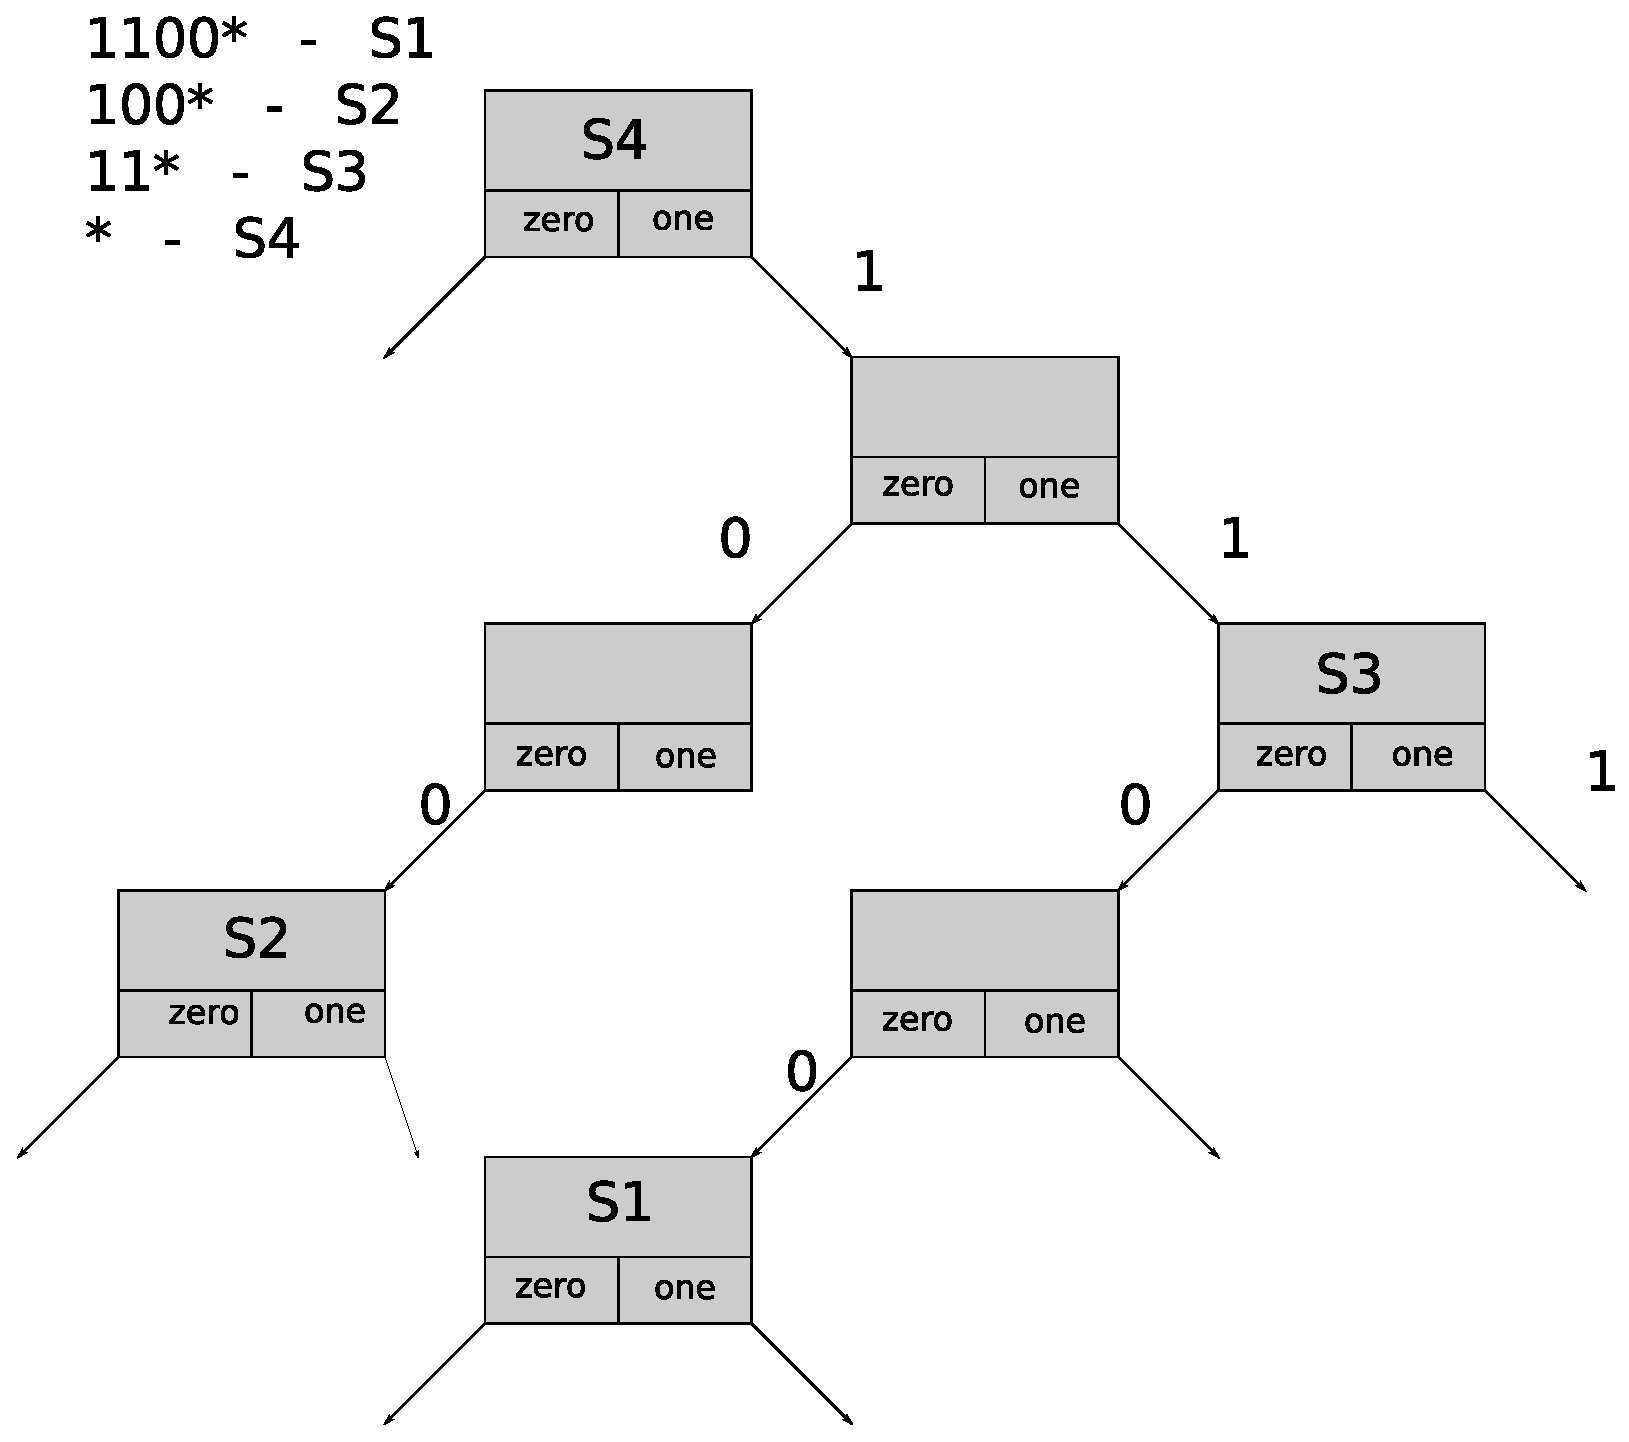
\includegraphics[scale=0.50]{4-implementacion/graf/lluinsert09.eps}
  \caption{Ejemplo de inserción de prefijos en árbol unibit}
  \label{fig:lluinsert}
\end{figure}

En la figura ~\ref{fig:lluinsert} se encuentra ejemplificada la inserción de 3 prefijos más la ruta por defecto. 

Comenzando por el nodo raíz, se inserta el prefijo 1100*. Para ello es necesaria la creación de 4 nodos hijos, uno por cada bit del prefijo. 

A continuación es insertado el prefijo 100*. Para el primer bit ya se encuentra creado el nodo, por lo cual se crean los 2 restantes necesarios.

Luego se inserta el prefijo 11*. Como anteriormente se había insertado el 1100* los nodos necesarios ya existen, por lo cual la inserción es trivial.

Por último en el nodo raíz se inserta la ruta por defecto (S4 en este ejemplo).

Tomando como ejemplo alguna dirección IP que comienza con 1100, puede verse que la búsqueda tomará el camino \textit{Raíz - one - one - zero - zero} y culminará en el nodo cuyo identificador de decisión es S1. 

Vale la pena considerar qué sucede si la dirección IP comienza con 1101. En este caso el camino que seguirá la búsqueda es \textit{Raíz - one - one - zero} y el puntero de recorrido quedará varado allí, ya que no existe en dicho punto un nodo asociado al puntero one. Vale recordar que en cada iteración, el algoritmo de búsqueda chequea si el nodo apuntado por el puntero de recorrido es decisión. Para este caso puede verse que en la segunda iteración (cuando se ha recorrido \textit{Raíz - one - one}) el algoritmo se encuentra parado en un nodo decisión y por lo tanto almacena el valor contenido en dicho nodo y procede a continuar. Cuando se encuentre varado en el próximo, lo que hará es retornar con el valor mencionado anteriormente. 

\subsection {Cache}

Se implementó una cache directa. La misma consta de una tabla hash de 16 entradas, aunque este tamaño puede ser modificado mediante la macro CACHE\_SIZE. Las colisiones se resuelven por reemplazo directo. La misma fue testeada con ambos algoritmos mencionados anteriormente. Para ello, se agregó una lógica adicional que consistió en:

\begin{itemize}
	\item Al tomar una dirección IP, chequear primero si el valor de decisión se encuentra en caché.
	\item Si está, retornar dicho valor.
	\item En otro caso, efectuar el lookup y almacenar el valor de decisión en caché. Para dicho almacenamiento, se efectúa un hash en la dirección IP, que consiste en calcular el resto de la división entre dicha dirección y el valor de CACHE\_SIZE. El resultado es utilizado como índice para el almacenamiento en la tabla.
\end{itemize}

Para evitar el overhead introducido por el uso de clases, se optó por una implementación basada en una estructura, a la cual se denominó \textit{HashEntry}. La misma cuenta con los siguientes campos:

\begin{itemize}
	\item address: Dirección IP almacenada.
	\item gw: Identificador de decisión.
	\item empty: Indica si la entrada de tabla está vacía.
\end{itemize}

\section{ISR}

Como se mencionó anteriormente, el módulo Uplink envía interrupciones al procesador. A fin de poder procesarlas en el software se implementó una ISR (Interrupt Service Routine) que hace uso de 3 elementos principales:

\begin{itemize}
	\item \textit{store\_array}: Es un buffer en el cual se van almacenando las palabras enviadas por el módulo Uplink.
	\item \textit{i}: Es un subíndice que sirve para moverse dentro del buffer anteriormente mencionado.
	\item \textit{flag}: Es un indicador que se incrementa cada vez que se produce una interrupción.
\end{itemize}

\textit{store\_array} está implementado como una matriz de enteros, y tiene 3 columnas. De esta manera, cada fila cuenta con con 96 bits de los cuales se utilizan 72 de ellos para almacenar las palabras enviadas por Uplink.

Cada vez que el procesador recibe una interrupción, lleva a cabo la lectura del valor recibido y la almacena en \textit{store\_array}, en el lugar indicado por \textit{i}. Luego el subíndice se incrementa, al igual que \textit{flag}.

En la función principal (main) existe una variable llamada \textit{flag2}. A ésta se le asigna el valor de \textit{flag}. Al producirse una interrupción, el valor de \textit{flag} se modifica y por lo tanto la condición de igualdad entre \textit{flag} y \textit{flag2} ya no se cumple. En ese momento se utilizan los valores almacenados en \textit{store\_array} para llevar a cabo el algoritmo de clasificación. Dichos valores a utilizar dependerán de la versión de Uplink que se esté utilizando:

\begin{itemize}
	\item Para la versión que envía quince palabras de 32 bits, es necesario esperar a la quinta palabra de 96 bits en \textit{store\_array} para poder localizar la dirección IP de destino, necesaria para realizar la clasificación. En la figura ~\ref{fig:ip15pal} se muestra cómo está localizada dicha dirección. 
	\item Para la versión que envía sólo una palabra de 32 bits, el procedimiento es trivial ya que esa misma palabra es la dirección IP de destino.
\end{itemize}


Una vez llevado a cabo el procedimiento de clasificación, \textit{flag2} es puesto de nuevo al valor de \textit{flag }y el proceso se repite.


\begin{figure}[H]
  \centering
	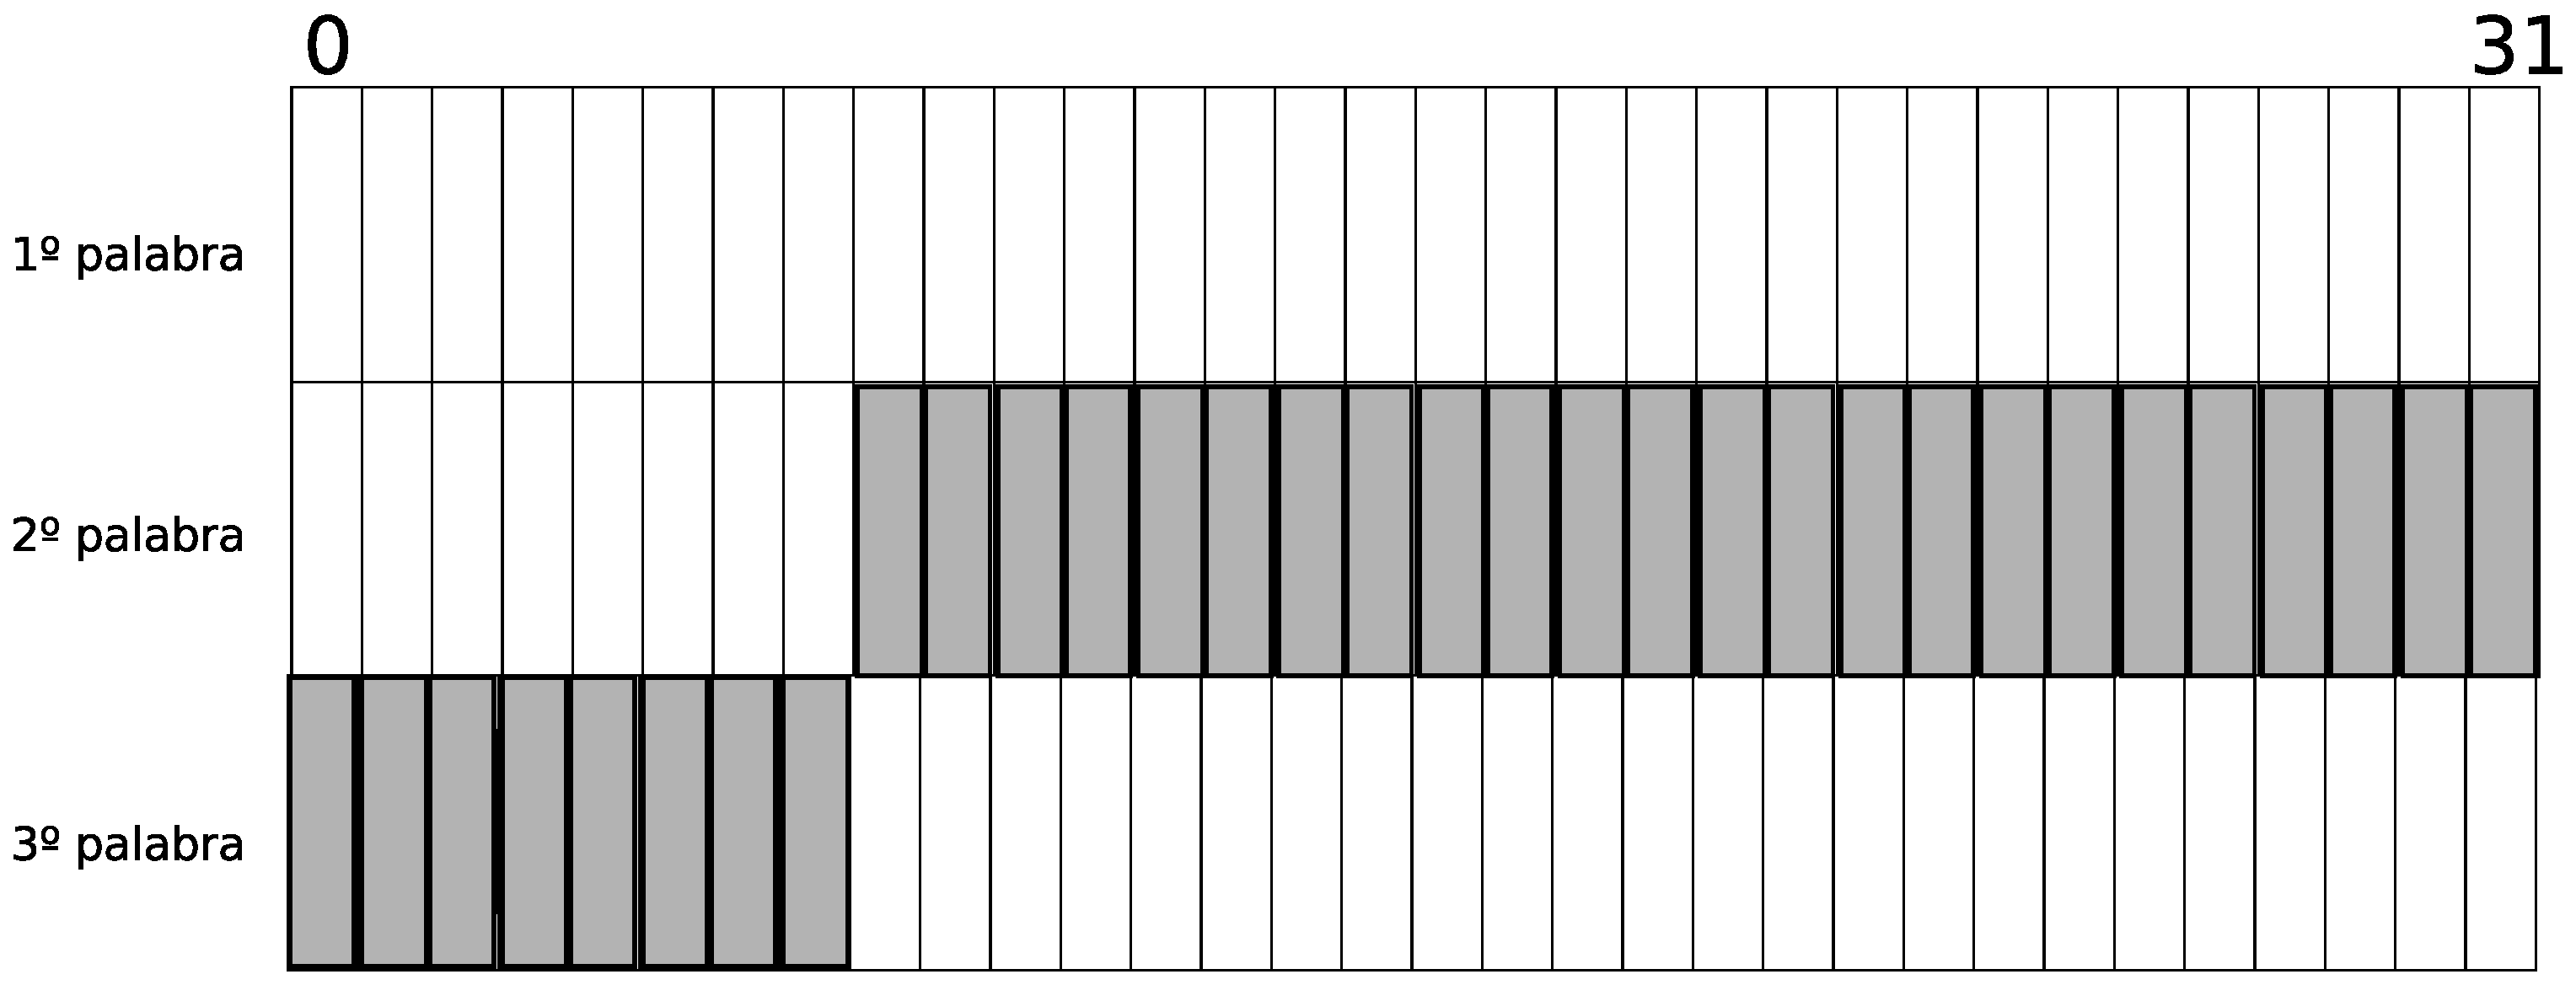
\includegraphics[scale=0.10]{4-implementacion/graf/ip15pal.eps}
  \caption{Ubicación de la dirección IP dentro de una palabra de 96 bits en store\_array, para la versión de Uplink que envía 15 palabras de 32 bits}
  \label{fig:ip15pal}
\end{figure}


\section{Hardware}

El hardware utilizado fue la placa de desarrollo DE2, cuyas características principales son:

\begin{itemize}
	\item FPGA: Cyclone II EP2C35F672C6
	\item USB Blaster integrado, para configuración de FPGA
	\item Memoria: 8 MB SDRAM, 512 KB SRAM, 4 MB Flash
	\item Clock de 50 MHz
\end{itemize}

Para una descripción más detallada, referirse al Apéndice A.

A su vez, la FPGA incluida en esta placa cuenta con estas características:

\begin{itemize}
	\item Elementos lógicos: 33216
	\item Bit totales de RAM: 483840
	\item Multiplicadores embebidos: 35
	\item PLLs: 4
	\item Cantidad máxima de pines definidos por el usuario: 475
\end{itemize}


\section{Microprocesador NIOS II}
El Nios II es un procesador RISC de 32 bits de propósito general que cuenta con las siguientes especificaciones:
\begin{itemize}
	\item Set de instrucciones, bus de datos y espacio de direcciones de 32 bits.
	\item 32 registros de propósito general.
	\item Soporte de hasta 32 interrupciones.
	\item Controlador de interrupciones externas para soportar una mayor cantidad de interrupciones.
	\item Multiplicación y división en una sola instrucción de 32 x 32 produciendo un resultado de 32-bits.
	\item Instrucciones dedicadas para multiplicaciones con resultados de 64 y 128 bits.
	\item Acceso a una variedad de periféricos e interfases a memorias  y periféricos fuera del chip.
	\item Modulo de depurado asistido por hardware.
	\item Unidad de manejo de memoria (MMU) opcional para soportar sistemas operativos mas complejos.
	\item Unidad de protección de memoria (MPU) opcional.
	\item Entorno de desarrollo de software basado en GNU C/C++ integrado a Eclipse.
	\item Integración con SignalTap® II, el analizador de lógica embebida de Altera permitiendo el análisis de tiempo real de todas las señales presentes en la FPGA.
	\item Set de instrucciones compatible entre todos las versiones del procesador Nios II.
\end{itemize}

Para poder ser implementado en una mayor variedad de dispositivos el Nios II ofrece 3 configuraciones diferentes:  Nios II/f (fast), Nios II/s (Standard), and Nios II/e (Economy).

\subsubsection{Nios II/e}
El Core Nios II/e esta diseñado para utilizar la menor cantidad de espacio posible. Esto esto funciona especialmente para FPGA de bajo costo. Tiene las siguientes características:
\begin{itemize}
	\item Espacio de direcciones de hasta 2GB
	\item Gratuito, no requiere licencia 
\end{itemize}

\subsubsection{Nios II/s}
El Nios II/s esta diseñado para mantener un balance entre rendimiento y costo. Entre sus características principales están:

\begin{itemize}
	\item Cache de instrucciones
	\item Espacio de direcciones de hasta 2GB
	\item Pipeline de 5 etapas
	\item Predictor de saltos estático
	\item Multiplicador y divisor por hardware. 
\end{itemize}

\subsubsection{Nios II/f}
El core Nios II/f esta diseñado para ofrecer la mayor performance a las expensas de un mayor tamaño, medido en unidades lógicas, este core tiene las siguientes características:

\begin{itemize}
	\item Cache de instrucciones y de datos separadas
	\item MMU y MPU opcionales
	\item Espacio de direcciones de hasta 2GB
	\item Pipeline de 6 etapas
	\item Multiplicador por hardware en un ciclo
	\item Divisor por hardware opcional
	\item Predictor de saltos dinámico
\end{itemize}

En vista de que este último ofrece la mayor performance y el hardware utilizado es capaz de soportarlo, se optó por el mismo para ser instanciado en el sistema.

\section{Verificación}
Se muestran a continuación varios casos de prueba que se realizaron para verificar el correcto funcionamiento del sistema.
\begin{table}
	\begin{tabular}{|>{\columncolor[gray]{0.8}}l|p{9cm}|} \hline
\multicolumn{2}{|>{\columncolor[gray]{0.8}}l|}{\textbf{Caso de Prueba: Funcionalidad del SoC}}\\ \hline
Propósito  & 1) Verificar la funcionalidad completa de System on Chip. 

2) Probar la correcta ejecución de software en el Nios II.

3) Comprobar el funcionamiento de las E/S del procesador. 
\\ \hline
 Prerrequisitos  & Se debe haber sintetizado el sistema completo y compilado sin errores el software.\\ \hline
 Datos de Prueba & Se preparara un sistema básico que incluye un Nios II/f, la interfaz de memoria y un PIO conectado a los LEDs de la placa.

Se usara un Software en C que va incrementando e imprimiendo en consola un valor entero mientras envía este valor, en binario, al PIO y por extensión a los LED.  \\ \hline
 Pasos & 1) Programar la FPGA con el sistema completo.

2) Descargar el Software al Microprocesador.

3) Iniciar la consola del NIOS II .\\ \hline
 Resultados Esperados & El valor del contador que se imprime por consola debe coincidir con el valor mostrado por los LED.\\ \hline
 Evaluación de la Prueba  & El resultado de la ejecución fue exitoso. \\ \hline
	\end{tabular}
	\caption{Caso de Prueba: Funcionalidad del SoC}
	\label{tab:testsoc}
\end{table}
\begin{table}
	\begin{tabular}{|>{\columncolor[gray]{0.8}}l|p{9cm}|} \hline
\multicolumn{2}{|>{\columncolor[gray]{0.8}}l|}{\textbf{Caso de Prueba: Interrupción, Envió y Recepción de datos}}\\ \hline
Propósito  & 1) Comprobar mediante un Custom Component simple el funcionamiento de las interrupciones.

2) Enviar y recibir un dato Estático por el bus sin errores. 
\\ \hline
 Prerrequisitos  & Se debe contar con el SoC Completo y funcional.\\ \hline
 Datos de Prueba & Se prepara un Componente propio simple que interrumpe, envía un dato y espera que el procesador le responda con le mismo dato. 

Preparar un software que cuente con la Rutina de Interrupción correspondiente y que cuando reciba un dato responda con el mismo de manera inmediata, además de imprimirlo por consola.
 \\ \hline
 Pasos & 1) Programar la FPGA con el sistema completo.

2) Descargar el Software al Microprocesador.

3) Iniciar la consola del NIOS II .
\\ \hline
 Resultados Esperados & En la consola debe aparecer repetidamente el valor que fue puesto en el Hardware. \\ \hline
 Evaluación de la Prueba  & El resultado de la prueba fue exitoso.\\ \hline
	\end{tabular}
	\caption{Caso de Prueba: Interrupción, Envió y Recepción de datos}
	\label{tab:enviorecepcion}
\end{table}
\begin{table}
	\begin{tabular}{|>{\columncolor[gray]{0.8}}l|p{9cm}|} \hline
\multicolumn{2}{|>{\columncolor[gray]{0.8}}l|}{\textbf{Caso de Prueba: Integridad del paquete }}\\ \hline
Propósito  & 1) Comprobar que la cabecera llega completa y sin errores al software. 

2) Verificar que el paquete sale del sistema completo.

3) Validar la correcta escritura del resultado en el tag Adjunto.

4) Comprobar que el paquete pasa sin errores por todo el sistema. 
\\ \hline
 Prerrequisitos  & Se debe contar con la Interfaz de acceso a la cabecera completa y funcional, el generador, el software necesario y se debe conectar la salida de Write Output a los LEDs de la placa .\\ \hline
 Datos de Prueba & Se configura el Generador con la cantidad que la cantidad de ciclos de reloj entre paquetes sea la máxima. 

Se prepara el software para que lea la cabecera completa, imprima lo leído en consola y responda automáticamente con un resultado conocido. 
 \\ \hline
 Pasos & 1) Programar la FPGA con el sistema completo.

2) Descargar el Software al Microprocesador.

3) Iniciar la consola del NIOS II .
\\ \hline
 Resultados Esperados & En la consola debe aparecer impresa la cabecera del paquete tal cual los valores predefinidos y en los LEDs debe aparecer al final de cada paquete el numero de paquete y el resultado conocido escrito.  \\ \hline
 Evaluación de la Prueba  & El resultado de la prueba fue exitoso.\\ \hline
	\end{tabular}
	\caption{Caso de Prueba: Integridad del paquete}
	\label{tab:integridad}
\end{table}
\begin{table}
	\begin{tabular}{|>{\columncolor[gray]{0.8}}l|p{9cm}|} \hline
\multicolumn{2}{|>{\columncolor[gray]{0.8}}l|}{\textbf{Caso de Prueba: Funcionamiento del LookUp }}\\ \hline
Propósito  & 1) Verificar que el lookup de direcciones se lleve a cabo exitosamente. 

\\ \hline
 Prerrequisitos  & Se debe contar con el software necesario para la clasificación de paquetes. Las pruebas se efectúan para cada algoritmo por separado. Se debe contar con un SoC que incluya un timer que luego será instanciado en el software para medir los retardos en el acceso.
 \\ \hline
 Datos de Prueba & Se generan dentro del mismo software una tabla de ruteo y otra tabla que contendrá las direcciones para efectuar el test. 

Se prepara el software para que imprima lo leído en consola. 
 \\ \hline
 Pasos & 1) Programar la FPGA con el sistema completo.

2) Descargar el Software al Microprocesador. 

3) Iniciar la consola del NIOS II .
\\ \hline
 Resultados Esperados & En la consola debe aparecer la dirección leída y el identificador de decisión para dicha dirección. \\ \hline
 Evaluación de la Prueba  & El resultado de la prueba fue exitoso.\\ \hline
	\end{tabular}
	\caption{Caso de Prueba: Retarde del Lookup}
	\label{tab:retlook}
\end{table}

\newpage
La figura ~\ref{fig:fpga} muestra el porcentaje de uso de los recursos de la FPGA utilizada para una FIFO con 4096 posiciones de memoria.
\begin{figure}[H]
  \centering
	\includegraphics[scale=0.70]{4-implementacion/graf/fpga.eps}
  \caption{Uso de los recursos de la FPGA}
  \label{fig:fpga}
\end{figure}

%\section{Distribucion Lineal}
 
\chapter{Resultados}

En este capitulo se presentan los resultados obtenidos de la ejecución del proyecto bajo ciertas condiciones representivas, con la intención de validar la funcionalidad y también de encontrar los puntos fuertes y las falencias del mismo.

\section{Configuración del Hardware}

\begin{center}
	\begin{longtable}{|l|p{4.75in}|} \hline
		\textbf{Feature} & \textbf{Description} \\ \hline
		FPGA & \begin{itemize}
			\item Cyclone II EP2C35F672C6 with EPCS16 16-Mbit serial configuration device.
			\end{itemize} \\ \hline
		I/O Interfaces &     \begin{itemize}
					\item Built-in USB-Blaster for FPGA configuration
    					\item Line In/Out, Microphone In (24-bit Audio CODEC)
   					\item Video Out (VGA 10-bit DAC)
   					\item Video In (NTSC/PAL/Multi-format)
   					\item RS232
    					\item Infrared port
   					\item PS/2 mouse or keyboard port
    					\item 10/100 Ethernet
   					\item USB 2.0 (type A and type B)
    					\item Expansion headers (two 40-pin headers)
				     \end{itemize} \\ \hline
		Memory & \begin{itemize}
					\item 8 MB SDRAM, 512 KB SRAM, 4 MB Flash
    					\item SD memory card slot
    			 \end{itemize} \\ \hline
		Displays & \begin{itemize}
					\item Eight 7-segment displays
    					\item 16 x 2 LCD display
    			 \end{itemize} \\ \hline
		Switches and LEDs & \begin{itemize}
					\item 18 toggle switches
    					\item 18 red LEDs
   					\item 9 green LEDs
   		 			\item Four debounced pushbutton switches
   				     \end{itemize} \\ \hline
		Clocks & \begin{itemize}
					\item 50 MHz clock
    					\item 27 MHz clock
   					\item External SMA clock input
   			 \end{itemize}	 \\ \hline
	\end{longtable} 
\end{center}

La FPGA incluida en la placa es una Cyclone II EP2C35 cuyas especificaciones son:

\begin{center}
	\begin{longtable}{|l|p{1.75in}|} \hline
		\textbf{Feature} & \textbf{Description} \\ \hline
		LEs & 33216 \\ \hline
		Total RAM bits & 483840 \\ \hline
		Embedded multipliers & 35 \\ \hline
		PLLs & 4 \\ \hline
		Maximum user I/O pins & 475 \\ \hline
	\end{longtable}
\end{center}

\subsection{Caso loopback}
\begin{figure}[h]
  \centering
	\includegraphics[width=0.70\textwidth]{5-resultados/graf/loop.eps}
  \caption{Caso Loopback para 1 y 15 palabras}
  \label{fig}
\end{figure}
En primera instancia nos ocupamos del caso loopback a los fines de encontrar los limites superiores de nuestro dise\~no.  En este caso, el software solo se limita a recibir los datos e inmediantemente después confirma el procesamiento y envía los resultados de regreso al hardware. Se realizan las pruebas correspondientes para las dos versiones de Uplink.
En el eje de las abscisas es posibles ver la cantidad de paquetes por segundo, el origen corresponde a la mayor velocidad a la que es posible transmitir sin perdidas. En las Ordenadas se puede observar la cantidad de paquetes perdidos en valores porcentuales, para obtener esta métrica se proceso una cantidad constante de paquetes, 9000, y luego se contrasto este valor con un contador global que el Generador estampa en la ultima palabra de cada paquete. Así se calculo la cantidad paquetes perdidos, sobre la cantidad total de paquetes generados. Este mismo sistema es el usado en todos los graficos posteriores.

\subsection{Caso Algoritmos unicamente}

Se estudiará la performance de los algoritmos aplicados, midiendo el retardo de lookup en funcion de la posición en la tabla de ruteo, se realizaran las pruebas de manera independiente al modulo extracto de cabeceras, para asi obtener una medida mas exacta del rendimiento.

\begin{figure}[h]
  \centering
	\includegraphics[width=0.8\textwidth]{5-resultados/graf/llu-utlsof.eps}
  \caption{Retardo de Busqueda LLU vs UTL}
  \label{fig}
\end{figure}

 
\chapter{Conclusiones}

En primer lugar, puede concluirse que existe factibilidad en la integración de módulos que realizan procesamiento de paquetes por hardware con aquellos que lo llevan a cabo por software.

Como se pudo ver en este trabajo la arquitectura utilizada es claramente modular y por lo tanto propicia para la integración de nuevos módulos. Esto último resulta fundamental por estos días debido a las crecientes necesidades en velocidad y ancho de banda.

Por otra parte, el hecho de no haber llevado a cabo pruebas con una interfaz de red real es compensado con el módulo \textit{ad-hoc} generador de paquetes, el cual brinda la posibilidad de generar tráfico Ethernet a la hora de realizar los testeos.

Se pudieron estudiar diversos algoritmos de clasificación para luego implementar 2 de ellos sobre una lógica reconfigurable y analizar comparativamente su performance.

Es posible efectuar mejoras en los esquemas implementados. Para el caso de una búsqueda lineal, puede implementarse una cola con prioridades para evitar el uso de templates y el overhead que ello implica. El el caso de la búsqueda en árbol puede optarse por un esquema multibit, que evite la expansión excesiva del árbol que contiene los prefijos 

\subsubsection{Trabajos Futuros}

Es posible realizar varias mejoras y extensiones a este proyecto, a continuación se muestra una lista de estas mejoras futuras:

\begin{itemize}
	\item asdsad
\end{itemize}






%\section{Distribucion Lineal}
 
\backmatter
\begin{thebibliography}{10}

\bibitem{netfpga} Website de NetFPGA: http://netfpga.org/

\bibitem{click} Website de Click Router: http://www.read.cs.ucla.edu/click/click

\bibitem{fifo} Open Cores. Proyecto Versatile FIFO:

http://opencores.org/project,versatile\_fifo

\bibitem{Varghese} George Varghese. \textit{Network Algorithmics: An interdisciplinary approach to designing fast networed devices}. Morgan Kaufmann Publishers. 2005 

\bibitem{CLassif}Yaxuan Qi, Jeffrey Fong, Weirong Jiang, Bo Xu, Jun Li, Viktor Prasanna. \textit{Multi-dimensional Packet Classification on FPGA: 100 Gbps and Beyond}. International Conference on Field-Programmable Technology (FPT '10), Pekín. 2010

\bibitem{jumbo} Greg Ferro. \textit{Ethernet Jumbo Frames, Full Duplex and Why Jumbo Frames Are 9000 Bytes}. 2011

\bibitem{terabit}Amit Singhal, Raj Jain. \textit{Terabit switching: a survey of techniques and current products}. Computer Communications, vol 25, pp 547-556. 2002.


\bibitem{Monta} Rogelio Montañana. \textit{El nivel de red en Internet}. 2011

\bibitem{niossw} Altera Corporation. \textit{NIOS II Software Developer's Handbook}. 2011.

\bibitem{nioshw} Altera Corporation. \textit{NIOS II Hardware Development Tutorial}. 2011.

\bibitem{sopc} Altera Corporation. \textit{SOPC Builder. User Guide}. 2011.

\bibitem{avalon} Altera Corporation. \textit{Avalon Interface Specifications}. 2011.

\bibitem{spaz} Santiago Paz, Jorge Finochietto, Carlos Zerbini. \textit{Diseño de Arquitectura Hardware Reconfigurable para la Conmutación de Paquetes en Redes Virtuales Privadas}. Proyecto integrador. 2011.



\end{thebibliography}.
%\section{Distribucion Lineal}

\chapter{Apéndice A}

\section*{Configuración del Hardware}

\begin{center}
	\begin{longtable}{|l|p{4.75in}|} \hline
		\textbf{Feature} & \textbf{Description} \\ \hline
		FPGA & \begin{itemize}
			\item Cyclone II EP2C35F672C6 with EPCS16 16-Mbit serial configuration device.
			\end{itemize} \\ \hline
		I/O Interfaces &     \begin{itemize}
					\item Built-in USB-Blaster for FPGA configuration
    					\item Line In/Out, Microphone In (24-bit Audio CODEC)
   					\item Video Out (VGA 10-bit DAC)
   					\item Video In (NTSC/PAL/Multi-format)
   					\item RS232
    					\item Infrared port
   					\item PS/2 mouse or keyboard port
    					\item 10/100 Ethernet
   					\item USB 2.0 (type A and type B)
    					\item Expansion headers (two 40-pin headers)
				     \end{itemize} \\ \hline
		Memory & \begin{itemize}
					\item 8 MB SDRAM, 512 KB SRAM, 4 MB Flash
    					\item SD memory card slot
    			 \end{itemize} \\ \hline
		Displays & \begin{itemize}
					\item Eight 7-segment displays
    					\item 16 x 2 LCD display
    			 \end{itemize} \\ \hline
		Switches and LEDs & \begin{itemize}
					\item 18 toggle switches
    					\item 18 red LEDs
   					\item 9 green LEDs
   		 			\item Four debounced pushbutton switches
   				     \end{itemize} \\ \hline
		Clocks & \begin{itemize}
					\item 50 MHz clock
    					\item 27 MHz clock
   					\item External SMA clock input
   			 \end{itemize}	 \\ \hline
	\end{longtable} 
\end{center}

La FPGA incluida en la placa es una Cyclone II EP2C35 cuyas especificaciones son:

\begin{center}
	\begin{longtable}{|l|p{1.75in}|} \hline
		\textbf{Feature} & \textbf{Description} \\ \hline
		LEs & 33216 \\ \hline
		Total RAM bits & 483840 \\ \hline
		Embedded multipliers & 35 \\ \hline
		PLLs & 4 \\ \hline
		Maximum user I/O pins & 475 \\ \hline
	\end{longtable}
\end{center}

\chapter{Apéndice B}

\section*{Bus Avalon}

Avalon es una familia de interfaces para flujo de datos de alta velocidad, lectura/escritura de registros y memoria, y control de dispositivos "off-chip". Existen varios tipos, cuyo uso depende de las necesidades del diseño a implementar:
\begin{itemize}
	\item Avalon ST: Soporta flujo unidireccional de datos, incluyendo flujos multiplexados y paquetes.
	\item Avalon MM: Interfaz de lectura/escritura basada en memoria, típica de conexiones maestro-esclavo.
	\item Avalon Conduit Interface: Para señales que no se amoldan a los tipos anteriores.
	\item Avalon TC: Para dispositivos "off-chip".
	\item Avalon Interrupt Interface: Permite el envío de interrupciones entre componentes.
	\item Avalon Clock Interface: Recibe y/o distribuye señales de clock.
	\item Avalon Reset Interface.
\end{itemize}

En el diseño correspondiente a este trabajo se optó por utilizar las siguientes interfaces:

\begin{itemize}
	\item Avalon MM, debido a que los componentes están mapeados en la memoria del sistema.
	\item Avalon Clock Interface, para proveer señal de reloj al sistema.
	\item Avalon Interrupt Interface, para el componente que requiere interrumpir al procesador.
\end{itemize}

\subsubsection{Avalon MM}
Las señales de dicha interfaz necesarias para este diseño son:

\begin{itemize}
	\item address: Direcciona los datos enviados hacia y recibidos desde el procesador.
	\item chipselect: Se usa en combinacion con read/write.
	\item read: Indica una transferencia de lectura.
	\item readdata: Los datos transferidos desde el periférico hacia el procesador.
	\item write: Indica una transferencia de escritura.
	\item writedata: Los datos trasferidos desde el procesador hacia el periférico. Debe tener el mismo ancho que readdata.

\end{itemize}

\subsubsection{Avalon CLock Interface}
En este caso, la señal necesaria es
\begin{itemize}
	\item clk: Provee clock para sincronización en lógica interna y otras interfaces.
\end{itemize}

\subsubsection{Avalon Interrupt Interface}
Para esta interfaz, la señal a utilizar es

\begin{itemize}
	\item irq: Permite al periférico enviar una señal de interrupción al procesador.
\end{itemize}

\chapter{Apéndice C}

\section*{Software}

\subsection*{NIOS II SBT}

El NIOS II Software Building Tools (o SBT) es un conjunto de utilidades y scripts que sirve para crear y construir aplicaciones embebidas basadas en C/C++, librerías de usuario y paquetes de soporte de placa (board support packages o BSP). 

Puede invocarse desde la IDE Eclipse o desde el intérprete de comandos del NIOS II.

El NIOS II SBT puede crear los siguientes tipos de proyecto:
\begin{itemize}
	\item Aplicación NIOS II: un programa que implementa alguna función deseada.
	\item NIOS II BSP: una librería que provee acceso al hardware en el sistema. Brinda un entorno de rutinas a medida para un procesador y, eventualmente, un sistema operativo. 
	\item Librería de usuario: un conjunto de funciones reutilizables. 
\end{itemize}

\subsubsection*{Aplicaciones y librerías de usuario}

Para el caso de aplicaciones y librerías de usuario, el SBT genera un makefile privado (denominado \textbf{Makefile}) el cual es usado para construir el proyecto. Al hacer esto se genera un archivo .elf para una aplicación, o .a para una librería. En este último caso, también se produce un makefile público (denominado \textbf{public.mk}), que se incluye en el privado para cualquier aplicación que use la librería de usuario.

Cuando se crea un makefile se provee al SBT con una lista de archivos de código fuente y una referencia al directorio donde se almacena el BSP. Luego, la herramienta examina la extensión de cada archivo fuente para determinar el lenguaje de programación. 

Actualmente los soportados son:

\begin{itemize}
	\item C (extensión .c).
	\item C++ (extensiones .cpp, .cxx, .cc).
	\item NIOS II Assembler (extensiones .s, .S).
\end{itemize}


\subsubsection{Board Support Packages}

Un BSP es una librería especializada que contiene código de soporte específico del sistema. Aisla la aplicación de los detalles del sistema, tales como mapeo de memoria, dispositivos disponibles y configuración del procesador.

Se compone de:

\begin{itemize}
	\item Capa de abstracción de Hardware (Hardware Abstraction Layer o HAL): Permite al software interactuar con el hardware del sistema. Se describirá en detalle más adelante en este capítulo.
	\item Librería C estándar newlib: ANSI C estándar diseñada para sistemas embebidos.
	\item Drivers de dispositivos: para manejar cada uno de los componentes del sistema.
	\item Paquetes de software opcionales: permiten proveer funcionalidad adicional.
	\item Sistema operativo de tiempo real opcional: implementación de MicroC/OS-II RTOS.
\end{itemize}

\subsubsection*{Proceso de construcción del software}

Para crear un proyecto de software se llevan a cabo una serie de pasos:

\begin{enumerate}
	\item Se obtiene el diseño de hardware sobre el cual va a correr el software. Dicha información está almacenada en un archivo de extensión \textbf{.sopcinfo}, el cual es generado por la herramienta SOPC builder.
	\item Se genera el BSP con las características necesarias según las funcionalidades requeridas. También se genera un makefile para dicho paquete.
	\item Opcionalmente, se crea una librería de usuario (junto a su correspondiente makefile).
	\item Se escribe el software de aplicación. Se colecta todo el código fuente, y luego se genera el makefile correspondiente.
	\item Se construye el proyecto.
\end{enumerate}


\subsection *{HAL}

La Capa de Abstracción de Hardware \textit{(Hardware Abstraction Layer o HAL)} provee una interfaz simple de drivers de dispositivos para conectar los programas con el hardware subyacente. La API está integrada con la librería estándar ANSI C, lo cual permite al software acceder a los dispositivos mediante el uso de funciones C ampliamente conocidas, tales como printf(), fopen(), fwrite(), etc.

\subsubsection*{Servicios}

La HAL provee los siguientes servicios:

\begin{itemize}
	\item Integración con la librería estándar newlib: provee funciones estándar ANSI C de amplio uso.
	\item Drivers de dispositivo: brinda acceso a cada dispositivo en el sistema.
	\item API: proporciona una interfaz estándar consistente a los servicios de la HAL, tales como acceso a dispositivos y manejo de interrupciones.
	\item Inicialización de sistema: Lleva a cabo la inicialización para el procesador y las rutinas antes de ejecutar la función principal (main).
	\item Inicialización de dispositivos: Instancia e inicializa cada uno de los dispositivos del sistema antes de que se ejecute la función main.
\end{itemize}

La figura ~\ref{fig:hal} muestra las capas de un sistema basado en la HAL, desde el nivel de hardware hasta el programa de usuario.

\begin{figure}[H]
  \centering
	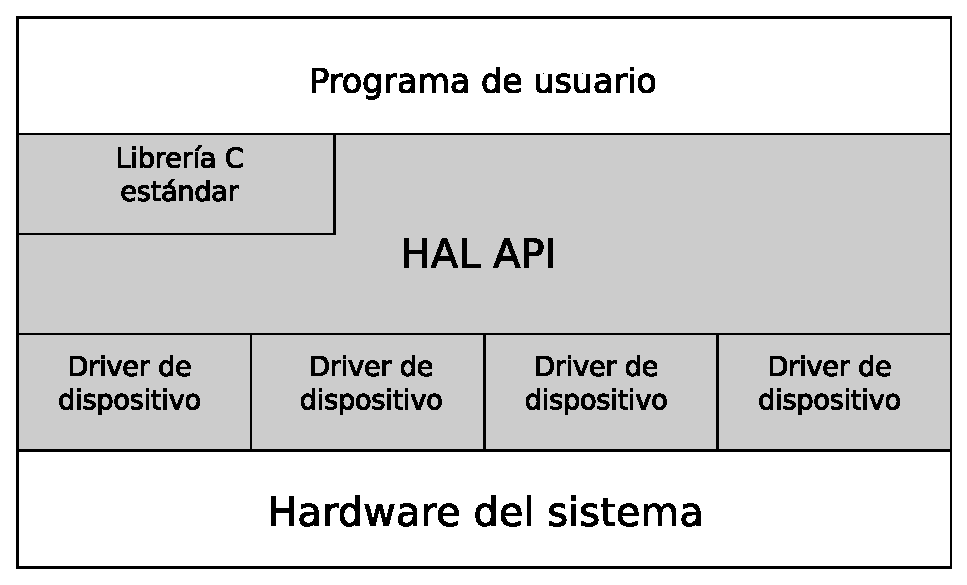
\includegraphics[width=0.80\textwidth]{3-arquitectura/graf/hal.eps}
  \caption{Capas de un sistema basado en la HAL.}
  \label{fig:hal}
\end{figure}

\subsubsection*{Modelos de dispositivos genéricos}

La HAL provee modelos de dispositivos genéricos para diversos tipos de periféricos que se encuentran en sistemas embebidos, tales como timers, interfaces Ethernet y dispositivos de I/O que transmiten datos de caracter. Estos modelos permiten escribir programas usando una API consistente sin preocuparse por el hardware subyacente.

Los tipos de periféricos cubiertos son:

\begin{itemize}
	\item Dispositivos de caracter: envían y/o reciben caracteres en forma serial, como ser una UART.
	\item Timers: dispositivos que llevan la cuenta de los tics de un clock y pueden generar interrupciones periódicas.
	\item Subsistemas de archivos: un mecanismo para acceder a archivos almacenados en dispositivos físicos. Dependiendo de la implementación interna, el driver del subsistema de archivos podría acceder a los dispositivos subyacentes en forma directa o usar un driver aparte.
	\item Dispositivos Ethernet: proveen acceso a una conexión Ethernet para una pila de red, tal como la NicheStack® TCP/IP Stack, provista por Altera.
	\item Dispositivos DMA: periféricos que llevan a cabo una gran cantidad de transacciones de datos. El origen y destino pueden ser la propia memoria o algún otro dispositivo.
	\item Dispositivos con memoria flash: periféricos con memoria no volátil que utilizan un protocolo especial de programación para almacenar datos.
\end{itemize}

Todos los periféricos, ya sean de Altera o de terceros, deben proveer un archivo de cabecera que defina la interfaz de bajo nivel del dispositivo con el hardware. 

Ciertos dispositivos tienen características específicas de hardware con requerimientos de uso que no se adaptan bien a una API de propósito general. La HAL maneja dichos requerimientos mediante la función ioctl(), cuyas opciones dependerán del periférico en cuestión.

Algunos periféricos proveen funciones de acceso dedicadas que no están basadas en el modelo genérico de la HAL. En ese caso, se debe proveer un archivo de cabecera con dichas funciones.


\subsubsection*{Librería C estándar : newlib}
La HAL integra su entorno de rutinas con una implementación open-source de la librería C estándar:\textbf{ newlib}. La misma está hecha para ser utilizada en sistemas embebidos. 

\subsubsection*{La HAL dentro de un proyecto de software}
La creación y administración de proyectos basados en la HAL están altamente ligadas al NIOS II SBT

\begin{figure}[h]
  \centering
	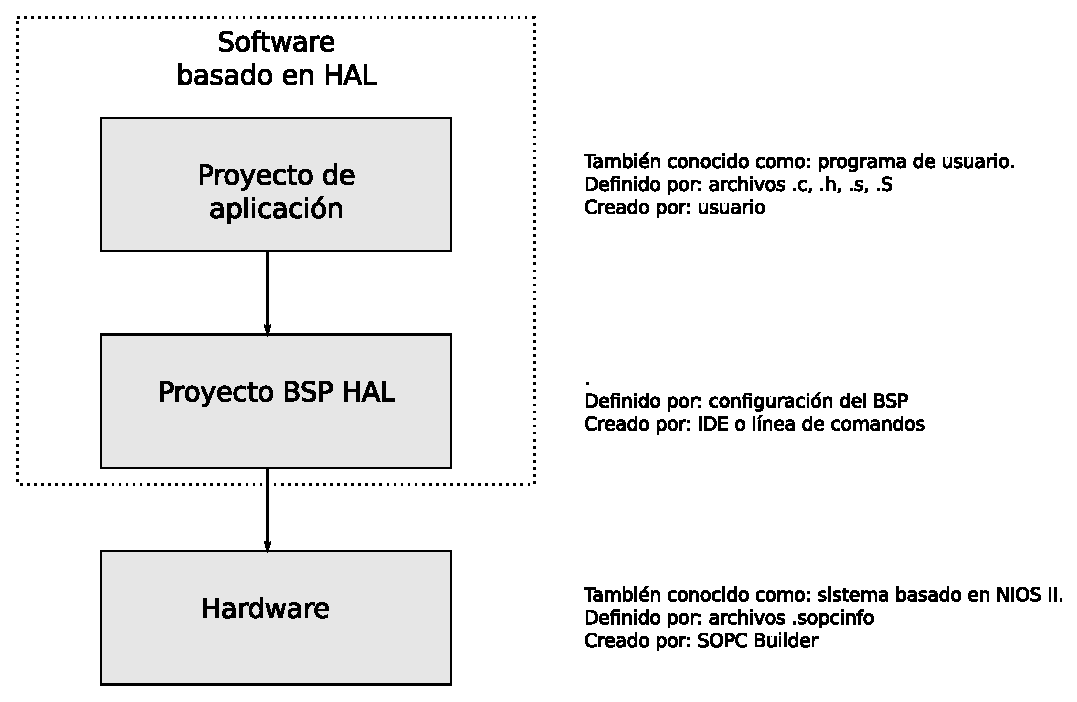
\includegraphics[width=0.90\textwidth]{3-arquitectura/graf/halsof.eps}
  \caption{Capas de un programa basado en HAL}
  \label{fig:halsof}
\end{figure}

La figura ~\ref{fig:halsof} muestra el diagrama en bloques de un software basado en la HAL. Todo programa de este tipo consta de dos proyectos. El código de aplicación específico se encuentra en uno de ellos, el cual depende a su vez de otro proyecto BSP separado.

EL primero contiene todo el código que el programador desarrolla. El segundo, toda la información necesaria para la interacción hardware-software. Este último a su vez depende del hardware del sistema, cuya información se encuentra en un archivo generado por la herramienta SOPC Builder.

\subsubsection*{El archivo de descripción del sistema (system.h)}
El archivo system.h provee una descripción completa del software del sistema basado en NIOS II. Describe cada periférico e incluye:

\begin{itemize}
	\item La configuración de hardware del periférico.
	\item La dirección base.
	\item Información IRQ (si es necesario).
	\item Un nombre simbólico para el periférico.
\end{itemize}

El SBT genera un archivo \textbf{system.h} para cada proyecto BSP, cuyo contenido dependerá del archivo .sopcinfo mencionado anteriormente en este capítulo.

\subsubsection*{Acceso al hardware}
El software accede al hardware a través de macros que abstraen la interfaz mapeada en memoria al dispositivo. Todos los componentes proveen un directorio que define el hardware y el software del periférico en cuestión. En esta carpeta se encuentra un archivo de cabecera que define la interfaz con el hardware y su nombre es $<componente>$\_regs.h, el cual se incluye en el subdirectorio inc. Por ejemplo, el componente JTAG UART define su interfaz en el archivo $<Directorio Instalacion Altera>$/ip/altera/sopc\_builder\_ip/

altera\_avalon\_jtag\_uart/inc/altera\_avalon\_jtag\_uart\_regs.h.

El archivo de cabecera \_regs.h define las siguientes macros de acceso para el componente:
\begin{itemize}
	\item Macros de acceso a registros que proveen operaciones de lectura/escritura. Éstas son:
	\begin{itemize}
		\item IORD\_$<NombreDelComponente>$\_$<NombreDelRegistro>$ ($<DireccionBaseDelComponente>$).
		\item IOWR\_$<NombreDelComponente>$\_$<NombreDelRegistro>$ ($<DireccionBaseDelComponente>$, $<Dato>$).
	\end{itemize}
	\item Macros de direccionamiento de registro, que retornan las direcciones físicas de cada uno de ellos. La dirección devuelta es la dirección base del componente + el valor de desplazamiento de registro especificado. Esta macro tiene el nombre de esta forma:
	\begin{itemize}
		\item IOADDR\_$<NombreDelComponente>$\_$<NombreDelRegistro>$ ($<DireccionBaseDelComponente>$).
	\end{itemize}
	\item Máscaras a nivel de bits. Estas macros tienen los siguientes nombres:
	\begin{itemize}
		\item $<NombreDelComponente>$\_$<NombreDelRegistro>$\_$<NombreDelCampo>$\_MSK : Máscara de bit de un campo.
		\item $<NombreDelComponente>$\_$<NombreDelRegistro>$\_$<NombreDelCampo>$\_OFST : Desplazamiento de bit del el comienzo del campo.
	\end{itemize}
\end{itemize}

Cabe mencionar que las los valores leídos/escritos mediante las macros de acceso a registro (IORD e IOWR) no trabajan con la caché del microprocesador.
En este contexto, es necesario destacar esto ya que los valores intercambiados entre el módulo software y el gestor de datos tienen que ser leidos/escritos solamente si estos están en el bus.

\chapter{Apéndice D}
\section*{SOPC Builder}

SOPC Builder es una herramienta que posibilita la definición y generación de Sistemas en Chips Programables (system-on-a-programable-chip, SOPC) en mucho menos tiempo que requieren los métodos manuales tradicionales de integración. Es parte del software Quartus II.

\subsection*{Componentes a medida (Custom Component)}

Además de una lista de componentes que ya están preparados para funcionar, SOPC Builder ofrece la posibilidad de crear componentes personalizados. Esto se efectúa importando módulos creados en algún HDL.

 Para integrarlos al diseño del sistema se siguen los siguientes pasos:
\begin{enumerate}
	\item Determinar las interfaces necesarias para interactuar con el componente.
	\item Crear la lógica del componente con algún HDL.
	\item Usar el editor de componentes de SOPC Builder para crear el componente a partir de los archivos HDL.
	\item Instanciar el componente en el sistema 
\end{enumerate}

\begin{figure}[H]
  \centering
	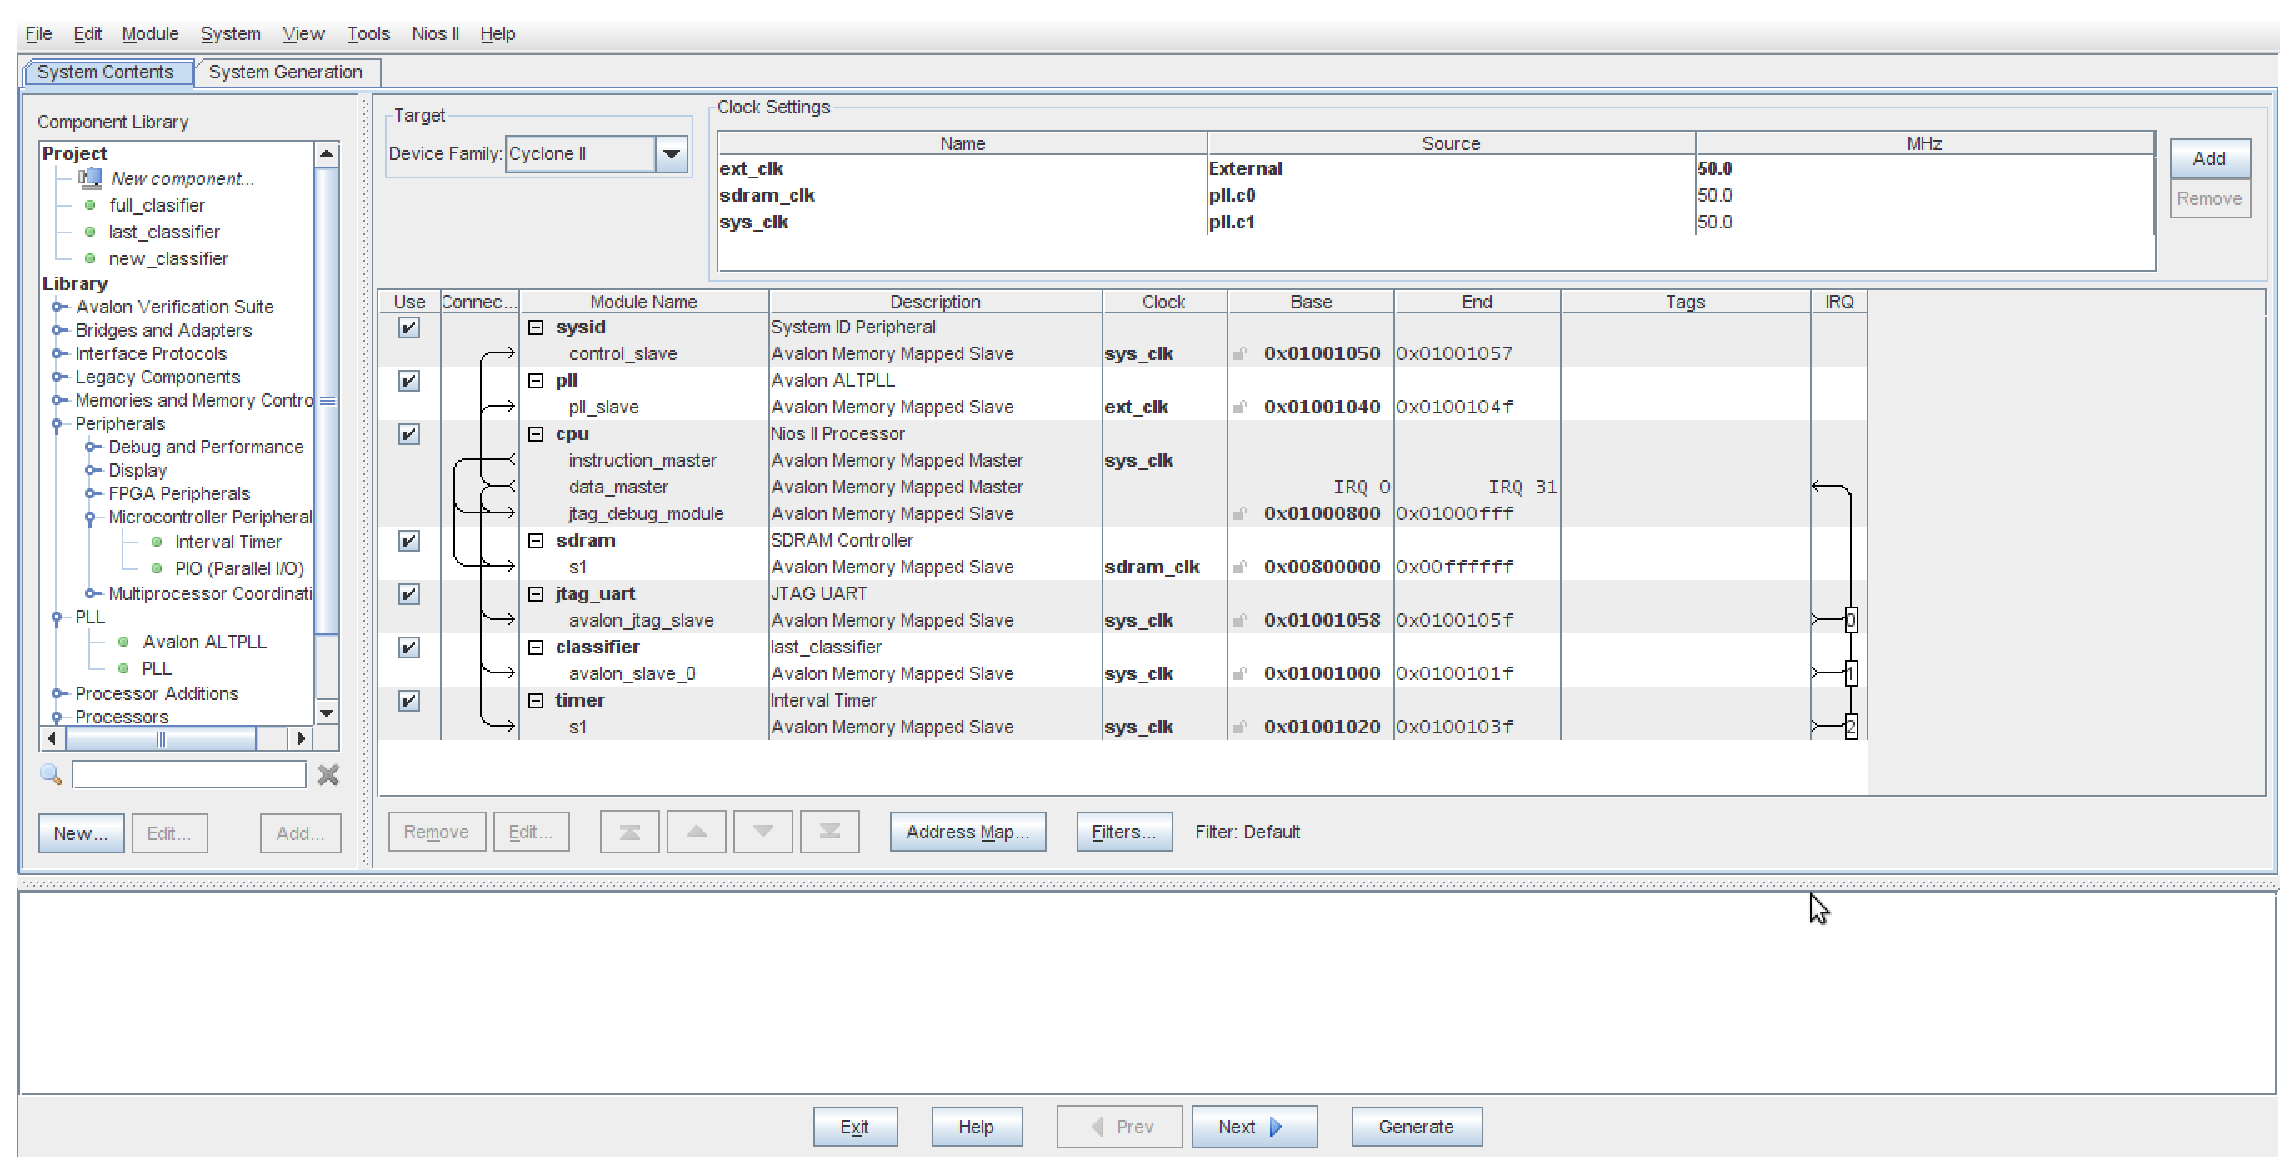
\includegraphics[width=0.90\textwidth]{8-apendices/graf/sopc1.eps}
  \caption{Ventana principal del SOPC Builder}
  \label{fig:sopc1}
\end{figure}

\begin{figure}[H]
  \centering
	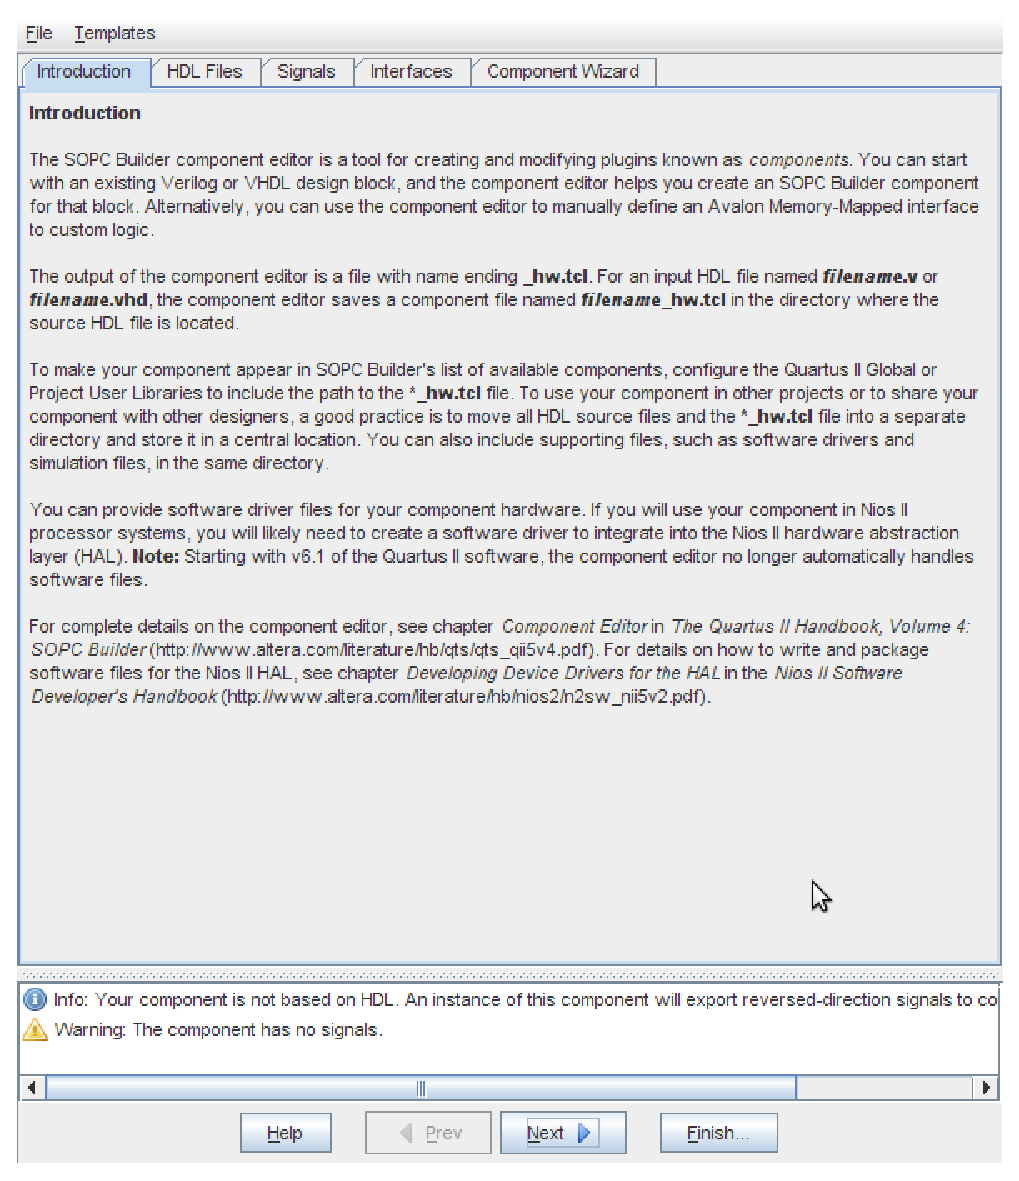
\includegraphics[width=0.60\textwidth]{8-apendices/graf/sopc2.eps}
  \caption{Generador de componentes}
  \label{fig:sopc2}
\end{figure}


\end{document}              % fin del documento
